\chapter{Fundamental Concepts for Early Detection of Multi-Stage APT Attacks}

\section{Introduction to Fundamental Concepts}
Modern cybersecurity faces increasingly sophisticated threats, particularly Advanced Persistent Threats (APTs). When 900 companies were surveyed about the most likely attacks on their business, APTs ranked at 57\% \cite{aag2024stats}. These threats require structured analysis frameworks to be understood and countered. The emergence of Machine Learning (ML) has introduced new dynamics and perspectives, serving both as a powerful tool for attackers to automate and personalize their operations, and for defenders to improve early detection and incident response. This chapter lays the conceptual foundations by examining these three essential pillars (APT, framework, ML) that support the development of an ML-augmented framework for detecting multi-stage APT attacks.

\section{Overview of Cybersecurity}

\subsection{Definition and Scope of Cybersecurity}
Cybersecurity is defined as the practice of protecting systems, networks, programs, and data from digital attacks, unauthorized access, damage, or destruction~\cite{cains2022cybersecurity,nist2023cyber}. It encompasses a broad set of technologies, processes, and practices designed to defend information assets across all layers of a digital environment --- from hardware infrastructure to software applications and human behavior~\cite{cisco2024cyber}.

The scope of cybersecurity extends across multiple domains, each addressing a distinct layer of protection~\cite{kang2023zero,cynet2023basics}:
\begin{itemize}
    \item \textbf{Network Security}: Protecting the integrity and usability of network infrastructure by preventing unauthorized access, misuse, or denial of service attacks.
    \item \textbf{Endpoint Security}: Securing individual devices such as computers, smartphones, and servers that connect to a network and serve as entry points for threats.
    \item \textbf{Application Security}: Ensuring that software applications are designed, developed, and maintained to resist exploitation of vulnerabilities.
    \item \textbf{Data Security}: Protecting the confidentiality, integrity, and availability of data --- whether stored, processed, or transmitted --- from unauthorized access or corruption.
    \item \textbf{Identity and Access Management (IAM)}: Controlling who has access to which resources, ensuring that only authorized users can interact with sensitive systems.
    \item \textbf{Cloud Security}: Addressing the unique risks of cloud environments, including misconfiguration, data breaches, and insecure interfaces.
    \item \textbf{Operational Security (OpSec)}: Managing the processes and decisions around handling and protecting data assets, including user behavior and access permissions.
\end{itemize}

\customexplication{A useful analogy is to think of cybersecurity as a multi-layered defense system --- similar to a medieval castle. The outer walls (network security) keep intruders out, the guards (endpoint and identity management) verify who enters, the vault (data security) protects the most critical assets, and internal surveillance (monitoring and logging) detects any suspicious activity that slips through.}

The field is commonly structured around three foundational principles, collectively known as the CIA Triad:
\begin{itemize}
    \item \textbf{Confidentiality}: Ensuring that information is accessible only to those authorized to access it.
    \item \textbf{Integrity}: Ensuring that data is accurate, consistent, and has not been tampered with.
    \item \textbf{Availability}: Ensuring that systems and data are accessible to authorized users when needed.
\end{itemize}

\customnote{These three principles --- Confidentiality, Integrity, and Availability --- serve as the evaluation criteria for nearly every security control and framework discussed throughout this document, including STRIDE, the Cyber Kill Chain, and MITRE ATT\&CK.}

As cyber threats have grown in sophistication, the scope of cybersecurity has expanded beyond purely technical concerns. Modern cybersecurity must address not only technological vulnerabilities, but also human factors such as social engineering, insider threats, and security awareness~\cite{chandel2017social}. This holistic view --- covering people, processes, and technology --- forms the foundation upon which advanced threat detection and response strategies, such as those discussed in subsequent sections, are built.

\subsection{Key Cybersecurity Concepts and Terminology}
A solid understanding of cybersecurity requires familiarity with its core vocabulary. The following concepts are foundational and appear throughout the literature, frameworks, and detection methodologies discussed in this document.

\begin{itemize}
      \item \textbf{Asset}: Any resource of value to an organization --- including hardware, software, data, networks, and personnel --- that must be protected from threats~\cite{hentea2021risk,huntress2024glossary}.
      \item \textbf{Threat}: Any potential event or action that could exploit a vulnerability to cause harm to an asset~\cite{huntress2024glossary}. Threats can be intentional (malicious attackers) or unintentional (human error, natural disasters).
      \item \textbf{Vulnerability}: A weakness or flaw in a system, application, or process that can be exploited by a threat actor. Vulnerabilities may exist in software code, system configurations, or organizational procedures~\cite{hentea2021risk}.
    \item \textbf{Exploit}: A specific method, tool, or piece of code that takes advantage of a vulnerability to cause unintended or unauthorized behavior in a system.
    \item \textbf{Risk}: The potential for loss or damage when a threat successfully exploits a vulnerability. Risk is commonly expressed as:
    \begin{center}
        $Risk = Threat \times Vulnerability \times Impact$
    \end{center}
      \item \textbf{Attack Surface}: The total sum of all possible entry points --- or attack vectors --- through which an unauthorized user could attempt to enter or extract data from a system. The larger the attack surface, the greater the exposure to potential threats~\cite{sentinelone2024vector}.
      \item \textbf{Attack Vector}: The specific path or method used by an attacker to gain unauthorized access to a system. Common vectors include phishing emails, unpatched software, weak passwords, and misconfigured cloud services~\cite{sentinelone2024vector}.
    \item \textbf{Threat Actor}: Any individual, group, or entity responsible for a security incident or attack. Threat actors are typically categorized by their motivation and capability:
    \begin{itemize}
        \item \textit{Nation-State Actors}: Highly skilled, state-sponsored groups conducting espionage or sabotage (e.g., APT groups).
        \item \textit{Cybercriminals}: Financially motivated individuals or organized groups.
        \item \textit{Insider Threats}: Employees or contractors who misuse their access, intentionally or accidentally.
        \item \textit{Hacktivists}: Groups motivated by political or ideological goals.
    \end{itemize}
\item \textbf{Indicator of Compromise (IoC)}: Evidence that a system has been breached or is under attack~\cite{crowdstrike2024ioa}. Common IoCs include unusual network traffic, unexpected file changes, unfamiliar processes, or suspicious login activity.
      \item \textbf{Indicator of Attack (IoA)}: Unlike IoCs --- which detect a breach after it occurs --- IoAs focus on detecting the behavior of an attack in progress, enabling earlier intervention before significant damage is done~\cite{crowdstrike2024ioa}.
\end{itemize}

\customexplication{A simple way to distinguish IoC from IoA: an IoC is like finding footprints left behind after a burglar has entered your house, while an IoA is like detecting the burglar trying to pick your lock before they get in. In the context of APT detection, IoAs are far more valuable because APTs are specifically designed to leave as few IoCs as possible.}

\begin{itemize}
      \item \textbf{Payload}: The component of malicious software (malware) that executes the intended malicious action --- such as encrypting files, stealing credentials, or establishing a backdoor --- once delivered to a target system~\cite{cloudflare2024payload}.
      \item \textbf{Zero-Day Vulnerability}: A software flaw that is unknown to the vendor and for which no patch or fix yet exists at the time of exploitation~\cite{deepinstinct2023zeroday}. Zero-day vulnerabilities are highly valuable to advanced threat actors, including APT groups, precisely because they cannot be detected by signature-based security systems.
\end{itemize}

\customnote{The Stuxnet attack --- referenced in Section 1.3 --- is one of the most documented examples of zero-day exploitation in history, relying on four simultaneous zero-day vulnerabilities to compromise its target.}

\begin{itemize}
      \item \textbf{Lateral Movement}: The techniques used by an attacker --- after gaining initial access to a network --- to progressively move through systems and gain access to higher-value targets~\cite{crowdstrike2024ioa}. Lateral movement is a defining characteristic of APT attacks and is further detailed in Sections 1.3 and 1.5.
      \item \textbf{Persistence}: The ability of an attacker to maintain long-term, undetected access to a compromised system, even after reboots or credential changes. Attackers achieve persistence through backdoors, scheduled tasks, or registry modifications.
      \item \textbf{Defense in Depth}: A layered security strategy that deploys multiple, overlapping security controls so that if one layer fails, others remain in place to prevent or detect an attack~\cite{cloudflare2024defense}. This principle underlies the multi-framework approach --- combining CKC, MITRE ATT\&CK, and Machine Learning --- explored throughout this document.
\end{itemize}

\subsection{Major Categories of Cyber Threats}
Cyber threats manifest in many forms, each with distinct mechanisms, objectives, and levels of sophistication. Understanding these categories is essential for designing effective detection and mitigation strategies. The following classification covers the most prevalent threat types encountered in modern cybersecurity environments~\cite{enisa2023threats}.

\textbf{Malware}\par
Malware (malicious software) is any software intentionally designed to disrupt, damage, or gain unauthorized access to a system. It represents one of the most common and diverse categories of cyber threats, and includes several subcategories:
\begin{itemize}
    \item \textbf{Viruses}: Malicious code that attaches itself to legitimate programs and spreads when executed.
    \item \textbf{Worms}: Self-replicating malware that spreads across networks without requiring user interaction.
    \item \textbf{Trojans}: Malicious programs disguised as legitimate software to deceive users into executing them.
    \item \textbf{Ransomware}: Malware that encrypts victim data and demands payment for the decryption key.
    \item \textbf{Spyware}: Software that secretly monitors user activity and exfiltrates sensitive information.
    \item \textbf{Rootkits}: Tools designed to hide the presence of malware or unauthorized access from detection systems.
\end{itemize}

\customnote{Ransomware has experienced significant industrialization in recent years, evolving from opportunistic attacks into coordinated, large-scale operations targeting critical infrastructure --- a trend discussed in detail in Chapter 2.}

\textbf{Social Engineering}\par
Social engineering attacks exploit human psychology rather than technical vulnerabilities, manipulating individuals into revealing confidential information or performing actions that compromise security~\cite{sentinelone2024social,akram2025social}. Key techniques include:
\begin{itemize}
    \item \textbf{Phishing}: Mass distribution of fraudulent emails designed to trick recipients into revealing credentials or clicking malicious links.
    \item \textbf{Spear Phishing}: A highly targeted form of phishing tailored to a specific individual or organization using personalized information.
    \item \textbf{Vishing}: Voice-based social engineering conducted via phone calls.
    \item \textbf{Pretexting}: Creating a fabricated scenario to manipulate a victim into providing information or access.
\end{itemize}

\customexplication{Spear phishing is the most commonly used technique for APT initial intrusion. As detailed in Section 1.3, APT actors invest significant resources in crafting convincing, personalized lures --- a capability that has been dramatically amplified by the integration of Generative AI, discussed in Chapter 2.}

\textbf{Denial of Service (DoS) and Distributed Denial of Service (DDoS)}\par
These attacks aim to make a system, service, or network unavailable to its intended users by overwhelming it with a flood of illegitimate requests~\cite{paloalto2024dos}. In a DDoS attack, this traffic originates from a large number of compromised devices (a botnet), making it significantly harder to mitigate. The targeted security property is Availability --- one of the three pillars of the CIA Triad.

\vspace{1em}
\textbf{Man-in-the-Middle (MitM) Attacks}\par
In a MitM attack, the attacker secretly intercepts and potentially alters communication between two parties who believe they are communicating directly with each other~\cite{hussain2023mitm,rapid72024mitm}. This allows the attacker to eavesdrop, steal credentials, or inject malicious content into the communication stream without either party's knowledge.

\vspace{1em}
\textbf{Insider Threats}\par
Insider threats originate from individuals within the organization --- such as employees, contractors, or business partners --- who misuse their authorized access to harm the organization. They are categorized as:
\begin{itemize}
    \item \textbf{Malicious Insiders}: Individuals who intentionally abuse their access for personal gain, espionage, or sabotage.
    \item \textbf{Negligent Insiders}: Users who unintentionally cause security incidents through careless behavior, such as clicking phishing links or mishandling sensitive data.
\end{itemize}

\textbf{Advanced Persistent Threats (APT)}\par
APTs represent the most sophisticated category of cyber threats. Unlike other attack types that seek immediate gains, APTs are characterized by stealth, persistence, and long-term strategic objectives --- such as espionage, sabotage, or data exfiltration~\cite{krishnapriya2024comprehensive}. APTs are typically conducted by nation-state actors or highly organized criminal groups with significant resources~\cite{crowdstrike2024apt}.

\customnote{Because APTs combine multiple threat categories --- malware, social engineering, lateral movement, and zero-day exploitation --- into a coordinated, multi-stage campaign, they require dedicated detection frameworks beyond standard security tools. This is precisely why Chapter 1 dedicates the following sections entirely to APT modeling, detection frameworks, and Machine Learning-based countermeasures.}

\textbf{Supply Chain Attacks}\par
Supply chain attacks target less-secure elements within a software or hardware supply chain to compromise a final, higher-value target. Rather than attacking an organization directly, the adversary infiltrates a trusted third-party vendor, software update mechanism, or component manufacturer to gain indirect access. Notable examples include the SolarWinds attack (2020), in which a compromised software update was distributed to thousands of organizations worldwide.

The taxonomy above illustrates that cyber threats vary greatly in complexity, origin, and intent. While traditional security tools are effective against known, lower-sophistication threats such as common malware and phishing, they fall short when facing multi-stage, adaptive attacks like APTs. This limitation motivates the adoption of structured frameworks and intelligent detection methods --- which form the core focus of this document.

\section{Advanced Persistent Threats (APT)}
\subsection{Definition and Characteristics}
The term \textbf{Advanced Persistent Threat (APT)} was introduced in 2006 by analysts at the United States Air Force (USAF) to describe intrusion activities that possessed specific characteristics \cite{singh2016comprehensive}. An APT is a targeted cyberattack that gains illegal access to information and communication systems with the aim of infiltrating and exfiltrating confidential data or harming an enterprise \cite{krishnapriya2024comprehensive}.

APTs are distinguished from traditional cybercriminal attacks by three main characteristics \cite{krishnapriya2024comprehensive,singh2016comprehensive}:
\begin{enumerate}
    \item \textbf{Advanced}: Attackers use sophisticated tools and techniques to bypass detection systems and maintain access to well-protected networks. The hacker is usually well-organized, adaptive in nature, and possesses significant resources \cite{singh2016comprehensive}.
    \item \textbf{Persistent}: The attacker demonstrates strong determination towards their target, using a slow process extended over time to achieve their objective. Persistence involves constantly collecting data from the target by exploiting various vulnerabilities \cite{krishnapriya2024comprehensive}. Even if the attacker achieves their initial goal, they persist within the system for further data exfiltration or to execute other significant changes.
    \item \textbf{Threat}: The attacker possesses the capability to access information, and the goal of the attack is often motivated by strategic advantages, industrial, military, or economic espionage, or political manipulation, rather than simple quick financial gains \cite{singh2016comprehensive}.
\end{enumerate}

\customexplication{As an analogy, consider two burglars: a direct attacker steals everything at once, ensuring immediate discovery. Conversely, an APT attacker discreetly copies the house key and secretly returns over time to steal small items sequentially. The key difference is the APT attacker's undetected persistence.}

The dwell time\footnote{Dwell time refers to the duration a cyber attacker remains undetected within a compromised network.} of APTs is often very long, highlighting the difficulty current detection systems have in identifying these stealthy attacks \cite{krishnapriya2024comprehensive}. APTs are generally implemented in several stages, often referred to as ``slow poisoning'' \cite{krishnapriya2024comprehensive}. They employ Tools, Techniques, and Procedures (TTPs) that are often novel and specifically developed to evade signature-based security systems\footnote{Signature-based security systems detect threats by comparing observed events against a database of known malicious patterns or ``signatures''.}. For example, the Stuxnet attack was particularly complex and remarkable because it relied on \textbf{four zero-day vulnerabilities\footnote{A zero-day vulnerability is a software flaw unknown to the vendor, meaning no patch exists when the attack occurs.}} simultaneously, digital signature forgeries, and deep knowledge of the target environment \cite{singh2016comprehensive}.

\customnote{The Stuxnet attack will be discussed in detail during the historical section of the ``Future Trends in Cyber Attacks'' chapter.}

\begin{figure}[H]
    \centering
    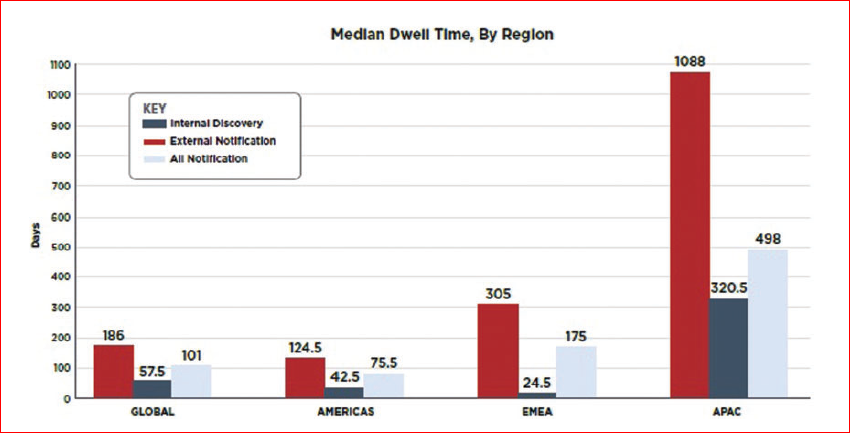
\includegraphics[width=0.7\textwidth]{figures/dwell}
    \caption{Dwell time in APT attacks}
    \label{fig:dwell}
\end{figure}

\subsection{Modeling APT Phases}
The APT attack process is inherently multi-stage. Although the exact number of steps may vary (some models describe four, five, six, or even eight), a typical APT lifecycle includes five essential phases for the majority of attacks \cite{krishnapriya2024comprehensive}:
\begin{enumerate}
    \item \textbf{Information Gathering (Reconnaissance)}: The attacker gathers information about the target organization, its resources, employees, and relationships, often via social engineering and passive web tools \cite{krishnapriya2024comprehensive}. This phase is crucial for developing attack tools and identifying the weakest link \cite{singh2016comprehensive}.
    \item \textbf{Initial Intrusion}: The adversary establishes a Point of Entry (POE) using social engineering techniques like \textbf{spear-phishing} (malicious email or link), water-hole attacks, or software vulnerability exploitation, often involving malware execution \cite{krishnapriya2024comprehensive}. Spear-phishing is the most commonly used technique for initial intrusion \cite{singh2016comprehensive}.
    \item \textbf{Command and Control (C\&C)}: A covert communication channel is established between the compromised host(s) and an external C\&C server. This communication must be maintained until the end of the attack and is essential for data transfer \cite{krishnapriya2024comprehensive}.
    \item \textbf{Lateral Movement}: The attacker attempts to move through the network by infecting more devices until reaching high-value targets, often using legitimate tools or reusing stolen credentials (credential dumping, pass-the-hash) \cite{krishnapriya2024comprehensive}.
    \item \textbf{Action on Objectives (AoO)}: The attacker achieves their ultimate goal, which may be data exfiltration, financial theft, system alteration (as in Stuxnet), or data destruction \cite{krishnapriya2024comprehensive}.
\end{enumerate}

\customwarning{It is important to note that different authors and experts may model APT phases differently. For example, some sources divide the attack into: Reconnaissance, Breach, Infiltration, Exfiltration, and Stealth Persistence. Because of these varying perspectives, the cybersecurity community emphasizes the need for standardized frameworks to provide a unified point of view.}

\begin{figure}[H]
    \centering
    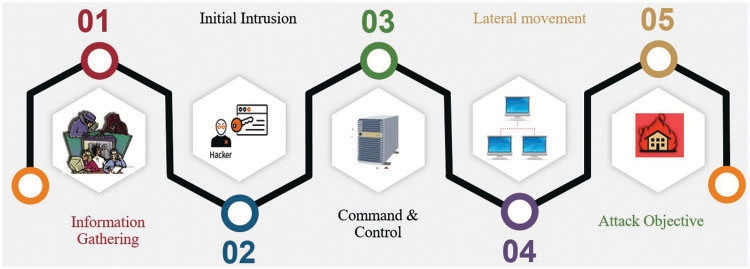
\includegraphics[width=0.8\textwidth]{figures/apt_steps}
    \caption{Stages of an APT attack}
    \label{fig:apt_steps}
\end{figure}

\section{Introduction to Threat Modeling Frameworks}

While the terms are often used as if they mean the same thing, there are actually three distinct categories of conceptual models used in cybersecurity. Each serves a different purpose in analyzing, classifying, and mitigating cyber threats— that is, taking protective measures to reduce, limit, or prevent the damage that cyber threats can cause. \cite{tatam2021review, huang2024security}.

\subsection{Category 1: Attack Lifecycle Models}
These models describe the stages of how an attack unfolds from start to finish \cite{tatam2021review, huang2024security}.
\begin{itemize}
    \item \textbf{Cyber Kill Chain:} Created by Lockheed Martin (2011), it outlines the 7 stages of an attack from reconnaissance to the final objective. It is formally defined as: reconnaissance, weaponization, delivery, exploitation, installation, command and control (C2), and actions on objectives (AoO) \cite{tatam2021review}.
    \item \textbf{MITRE ATT\&CK:} Created by MITRE (2013), it details the tactics and techniques of real attackers based on real-world incidents \cite{jiang2025mitre, tatam2021review}. Organized into three technology domains---Enterprise (traditional networks and cloud technologies), Mobile (mobile devices), and ICS (Industrial Control Systems)---it maps specific adversarial tactics (high-level objectives) and techniques (specific actions) that describe how an attacker seeks to compromise or persist in a system \cite{jiang2025mitre}.
    \item \textbf{Unified Kill Chain:} Created by Paul Pols (2017), this is an extended version that includes  18 phases, offering more detail than the traditional Kill Chain. It was developed by combining and extending the Cyber Kill Chain with the MITRE ATT\&CK framework \cite{tatam2021review}.
\end{itemize}

\customnote{The Cyber Kill Chain and the MITRE ATT\&CK framework will be discussed in detail in different sub-parts, as they represent the core of threat detection methods and are some of the most widely used frameworks.}

\subsection{Category 2: Threat Modeling Frameworks}
These frameworks help security professionals analyze and classify threats during the system design phase \cite{huang2024security, ouaissa2025smartcity}. Threat modeling is a proactive approach used primarily in the early stages of a system's lifecycle to anticipate potential cybersecurity threats and vulnerabilities, enabling the incorporation of relevant mitigation controls into the system design \cite{huang2024security, owasp2024threatmodeling}.
\begin{itemize}
    \item \textbf{STRIDE:} Classifies threats into 6 types: Spoofing, Tampering, Repudiation, Information Disclosure, Denial of Service (DoS), and Elevation of Privilege. First introduced to developers at Microsoft in 1999, STRIDE is a system/software-based taxonomy for identifying threats based on their explicit type \cite{tatam2021review, ouaissa2025smartcity}.
    \item \textbf{PASTA:(Process for Attack Simulation and Threat Analysis)}a seven-step threat modeling methodology that integrates business objectives and technical requirements to deliver a comprehensive, risk-based assessment of potential threats. Unlike other methodologies focused exclusively on technical vulnerabilities, PASTA let's you adopts  the whole approach that considers both business impact and technological concerns \cite{ouaissa2025smartcity}.
    
    \begin{figure}[H]
        \centering
        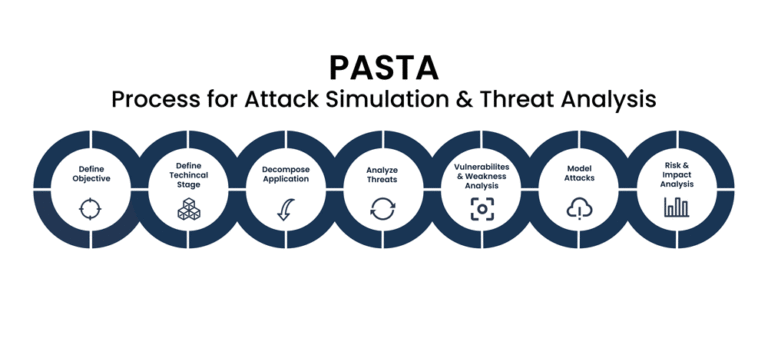
\includegraphics[width=0.7\textwidth]{figures/PASTA.png}
        \caption{Steps of the PASTA methodology}
        \label{fig:pasta}
    \end{figure}

    \item \textbf{DREAD:} Rates threats by 5 categories: Damage potential, Reproducibility, Exploitability, Affected users, and Discoverability. Initially established as part of Microsoft's Security Development Lifecycle (SDL), it has since become a widely adopted approach for risk prioritization across a variety of sectors \cite{ouaissa2025smartcity}.
    \item \textbf{VAST:} Built specifically for large-scale enterprises and agile/DevOps environments, it provides a scalable threat modeling approach suitable for complex organizational contexts \cite{tatam2021review, ouaissa2025smartcity}.
    \item \textbf{Attack Trees:} A visual tree structure mapping all possible paths to achieve an attack goal. Attack Trees formally identify and define the variety of attacks a system can be subjected to, representing them in a hierarchical structure where the root node signifies the attacker's goal and the leaf nodes depict all possible paths to fulfill that objective \cite{tatam2021review}.
    
    \begin{figure}[H]
        \centering
        \includegraphics[width=0.7\textwidth]{"figures/tree-attack.png"}
        \caption{Example of an Attack Tree structure}
        \label{fig:attack_tree}
    \end{figure}
\end{itemize}

\subsection{Category 3: Adversary Behavior \& Incident Analysis Models}
These models focus on understanding who the attacker is, how they operate, and assisting in incident analysis \cite{tatam2021review, huang2024security}.
\begin{itemize}
    \item \textbf{Diamond Model:} Focuses on the interaction between four fundamental elements: adversary, victim, infrastructure, and capabilities. It is widely used to track attack groups and model intrusion flows. \cite{tatam2021review, huang2024security}.
    \item \textbf{MITRE D3FEND:} The defensive counterpart to ATT\&CK, which maps defensive countermeasures to attack techniques. D3FEND has been integrated with ATT\&CK-based defense strategies, for example against IoT botnet attacks within smart city environments, showcasing the practical utility of combining MITRE offensive and defensive frameworks \cite{jiang2025mitre}.
    \item \textbf{TIBER-EU:} A European framework designed for simulating real Advanced Persistent Threat (APT) attacks on financial institutions, providing a structured methodology for red-team testing and threat intelligence-led adversarial simulations in the financial sector.
\end{itemize}

\customexplication{Each framework category acts as a specific tool serving a distinct phase of the attack timeline. Pre-incident, Category 2 (Threat Modeling) is used to design resilient systems that are not easily bypassed. During an incident, Category 1 (Attack Lifecycle) serves to trace and detect the stages of an active attack. Finally, post-incident, Category 3 (Adversary Behavior) is essential for investigating the attack and profiling the attacker's methods.}

\section{The Cyber Kill Chain (CKC)}
\subsection{Structure and Objective of the Model}
The Cyber Kill Chain (CKC), developed by Lockheed Martin, is a conceptual framework that describes the sequence of steps typically followed by cyber intruders to achieve their goal \cite{singh2016comprehensive, ahmed2021cyber}. This model helps cybersecurity professionals identify and mitigate threats by decomposing the attack lifecycle into discrete phases, allowing for more targeted and effective defense measures. The CKC model has been widely used to analyze APT campaigns, providing a taxonomy based on the adversary's TTPs \cite{jiang2025mitre, ahmed2021cyber}.

\subsection{Detailed Description of the Seven Phases}
The CKC model consists of seven distinct stages, the execution of which in an uninterrupted sequence is necessary for the success of the attack \cite{singh2016comprehensive, ahmed2021cyber}:
\begin{enumerate}
    \item \textbf{Reconnaissance}: The attacker performs research on the target to identify systems, employees, and exploitable vulnerabilities \cite{krishnapriya2024comprehensive}.
    \item \textbf{Weaponization}: The attacker couples malware (such as a Remote Access Trojan - RAT) with an exploit code (exploit kit) into a deliverable payload, such as PDF or Microsoft Office files \cite{singh2016comprehensive}.
    \item \textbf{Delivery}: The payload is transmitted to the target, often via email (phishing), compromised websites, or removable media \cite{singh2016comprehensive}.
    \item \textbf{Exploitation}: Once the payload is successfully delivered, a vulnerability is exploited to execute malicious code on the target system \cite{singh2016comprehensive}.
    \item \textbf{Installation}: The attacker installs persistent access points (e.g., backdoors or persistence mechanisms) to guarantee continuous access to the system or network \cite{singh2016comprehensive}.
    \item \textbf{Command and Control (C\&C)}: The adversary establishes a communication channel with the compromised host to manipulate the cyber weapon and guide actions remotely \cite{krishnapriya2024comprehensive}.
    \item \textbf{Action on Objectives (AoO)}: The attacker realizes their final objective, such as data theft, encryption, or information destruction \cite{krishnapriya2024comprehensive}.
\end{enumerate}

\begin{figure}[H]
    \centering
    \includegraphics[width=0.9\textwidth]{"figures/The 7 Steps -ckc.png"}
    \caption{The 7 Steps of the Cyber Kill Chain (CKC)}
    \label{fig:ckc_7steps}
\end{figure}

\section{The MITRE ATT\&CK Framework}
\subsection{Fundamental Concepts and Structure}
MITRE ATT\&CK (Adversarial Tactics, Techniques, and Common Knowledge) is a structured knowledge base describing cyber adversary behavior across various domains (enterprise, mobile, industrial control systems - ICS) \cite{jiang2025mitre}. Developed in 2013, it serves as a fundamental basis for mapping adversary Tactics, Techniques, and Procedures (TTPs) \cite{jiang2025mitre}.

The framework's structure revolves around four main components \cite{jiang2025mitre}:
\begin{enumerate}
    \item \textbf{Tactics}: The adversary's high-level objectives (similar to CKC phases, but more numerous and detailed).
    \item \textbf{Techniques}: The specific methods used to achieve these objectives.
    \item \textbf{Sub-techniques}: Detailed methods that break down techniques.
    \item \textbf{Documented Usage}: Associated procedures and metadata.
\end{enumerate}
ATT\&CK is organized into matrices representing adversary operating environments: \textbf{Enterprise} (traditional networks and cloud), \textbf{Mobile}, and \textbf{ICS} \cite{jiang2025mitre}.

\begin{figure}[H]
    \centering
    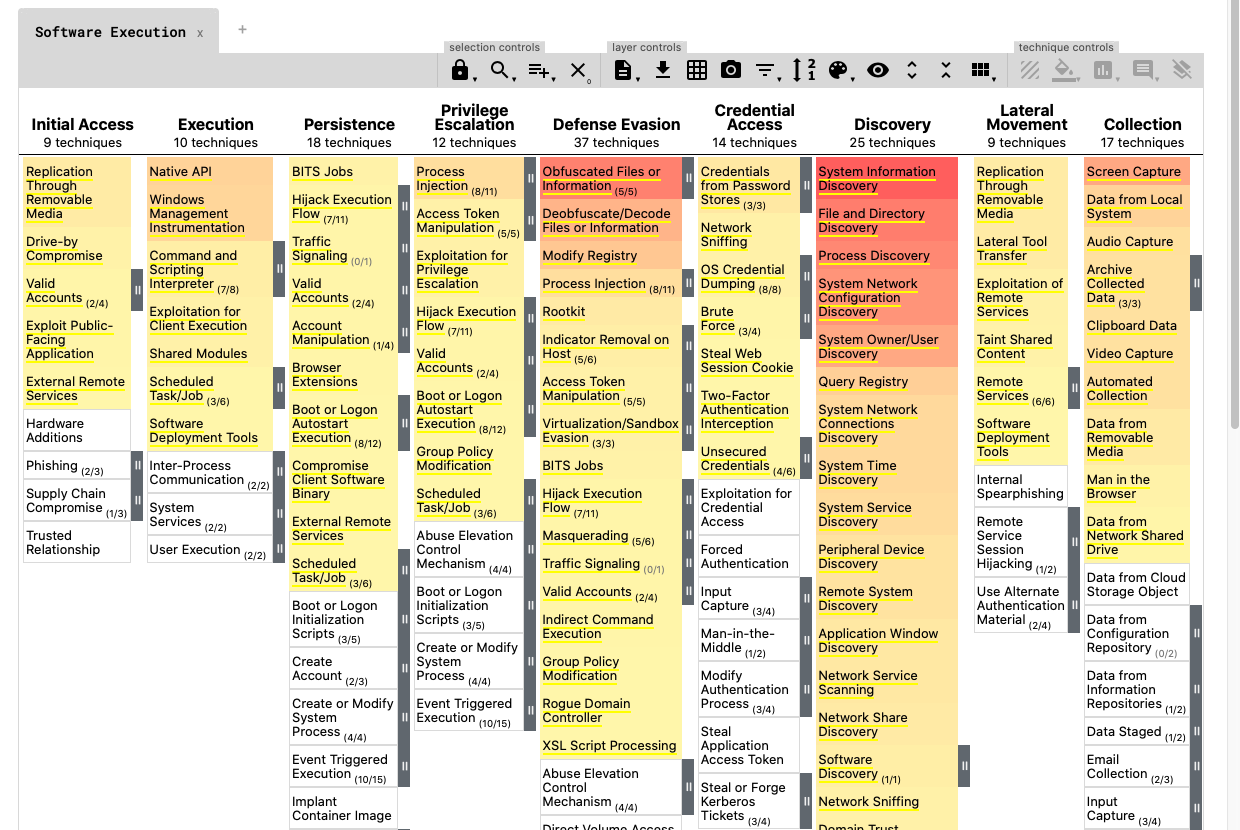
\includegraphics[width=0.9\textwidth]{figures/MITRE.png}
    \caption{The MITRE ATT\&CK Framework matrix}
    \label{fig:mitre_framework}
\end{figure}

\subsection{Applications and Integration with CKC}
MITRE ATT\&CK is a widely adopted tool for strengthening cybersecurity, notably by supporting Cyber Threat Intelligence (CTI), incident response, attack modeling, and vulnerability prioritization \cite{jiang2025mitre}.

\textbf{APT Detection}: One of the fundamental uses of ATT\&CK is improving the systematic detection and analysis of threats, particularly APTs \cite{jiang2025mitre}. The framework is used to model APT attack footprints using TTP-based attack trees. Coverage percentage relative to ATT\&CK is even used as a metric to evaluate the performance of APT detection models\footnote{\textbf{What is ATT\&CK Coverage Percentage as a Metric?} When researchers build an APT detection model, they measure how many ATT\&CK techniques their model can detect. The coverage percentage tells you: "Out of all the known attack techniques in the ATT\&CK framework, how many can this model catch?" — a higher percentage means the model is better at detecting a wider range of attacks.}. Studies identify that the most frequently observed tactics are Initial Access (especially Spearphishing Link at 45.5\%), Execution, and Discovery \cite{jiang2025mitre, cisa202x}.

\textbf{CKC/ATT\&CK Integration}: ATT\&CK is often integrated with other frameworks like the Cyber Kill Chain. While CKC offers a sequential view of the attack, ATT\&CK provides the granularity of TTPs at each stage \cite{jiang2025mitre}. Integration fills the gaps in CKC, which lacks detailed information on adversary tactics and techniques. This complementarity is vital for early detection, as it maps adversary actions to different CKC phases \cite{jiang2025mitre}.

\customexplication{If the Kill Chain provides the chapter headings, ATT\&CK provides the detailed content for each chapter.}

\section{Introduction to Machine Learning}

\subsection{Definition and Core Concepts of Machine Learning}

Machine Learning (ML) is a subfield of Artificial Intelligence (AI) that enables computer systems to learn from data and improve their performance on a given task without being explicitly programmed to do so. Rather than following a fixed set of rules written by a programmer, an ML model identifies patterns, relationships, and regularities within data, and uses this learned knowledge to make predictions or decisions on new, unseen data.

Formally, the learning process can be described as follows: given a set of training examples, an ML algorithm adjusts its internal parameters to minimize the difference between its predictions and the actual outcomes --- a process known as optimization. The quality of this learning is measured using a loss function, which quantifies how far the model's predictions are from the true values.

\subsubsection*{Explication}
A helpful analogy: teaching a child to recognize cats does not involve giving them a precise list of rules (``four legs, pointed ears, fur''). Instead, you show them hundreds of examples of cats and non-cats, and they gradually learn to distinguish them on their own. Machine Learning works in exactly the same way --- it learns from examples rather than from explicit instructions.

\subsubsection*{Core Concepts}

\begin{description}
    \item[Training Data] The dataset used to teach the model. It consists of input examples (features) and, in supervised settings, their corresponding correct outputs (labels). The quality, quantity, and diversity of training data directly determine the quality of the learned model.
    
    \item[Features] The individual measurable properties or characteristics of the data used as inputs to the model. Feature selection and engineering --- the process of choosing and transforming the most relevant features --- is one of the most critical steps in building an effective ML model.
    
    \item[Model] A mathematical function or structure that maps input data to an output prediction. The model's internal parameters are adjusted during training to best fit the patterns observed in the training data.
    
    \item[Training and Testing] The dataset is typically split into:
    \begin{itemize}
        \item \textbf{Training set}: Used to fit the model's parameters.
        \item \textbf{Validation set}: Used to tune hyperparameters and monitor learning during training.
        \item \textbf{Test set}: Used to evaluate the model's final performance on completely unseen data.
    \end{itemize}
    
    \item[Overfitting and Underfitting] Two fundamental challenges in ML model development:
    \begin{itemize}
        \item \textbf{Overfitting} occurs when a model learns the training data too well --- including its noise and irrelevant details --- resulting in poor generalization to new data.
        \item \textbf{Underfitting} occurs when a model is too simple to capture the underlying patterns in the data, resulting in poor performance on both training and test data.
    \end{itemize}
    
    \textbf{Note:} Overfitting is a particularly significant concern in cybersecurity applications of ML, where models must generalize to novel, previously unseen attack patterns rather than simply memorizing known ones.
    
    \item[Hyperparameters] Configuration settings defined before training begins --- such as learning rate, number of layers, or number of trees --- that control the learning process itself, as opposed to the model parameters learned from data.
    
    \item[Generalization] The ability of a trained model to perform well on new, unseen data that was not part of the training set. Generalization is the ultimate goal of any ML model, and is especially critical in dynamic environments such as cybersecurity, where threat patterns evolve continuously.
    
    \item[Loss Function and Optimization] The loss function measures how far the model's predictions deviate from the true labels. The training process seeks to minimize this loss using optimization algorithms --- the most common being Gradient Descent and its variants (e.g., Adam, SGD), which iteratively adjust model parameters in the direction that reduces the loss.
    
    \item[Evaluation Metrics] Once trained, a model's performance is assessed using metrics appropriate to the task:
    \begin{itemize}
        \item \textbf{Accuracy}: The proportion of correct predictions out of all predictions.
        \item \textbf{Precision}: The proportion of true positive predictions among all positive predictions.
        \item \textbf{Recall (Sensitivity)}: The proportion of actual positives correctly identified by the model.
        \item \textbf{F1-Score}: The harmonic mean of precision and recall, balancing both metrics.
        \item \textbf{AUC-ROC}: A measure of the model's ability to distinguish between classes across all classification thresholds.
    \end{itemize}
\end{description}

\subsubsection*{Explication}
In cybersecurity and APT detection specifically, \textbf{Recall} is often prioritized over \textbf{Accuracy}. Missing a real attack (a false negative) is far more costly than incorrectly flagging a benign event (a false positive). A model that detects 99\% of attacks while generating some false alarms is far preferable to one that misses critical threats.

Machine Learning's ability to detect complex, non-linear patterns in large datasets makes it particularly well-suited for cybersecurity applications --- a capability that static, rule-based systems fundamentally lack. The following sections elaborate on the different learning paradigms ML employs, and on how these capabilities are harnessed to detect sophisticated threats such as APTs.

\subsection{Domains and Learning Paradigms}

Machine Learning is not a single, uniform approach --- it encompasses several distinct learning paradigms, each defined by the type of data available and the nature of the task to be solved. Understanding these paradigms is essential, as different cybersecurity problems require different learning strategies. Additionally, ML operates across a range of application domains, each contributing specific capabilities to threat detection and analysis.

\subsubsection*{Learning Paradigms}

\begin{description}
    \item[Supervised Learning] Supervised learning is the most widely used ML paradigm. The model is trained on a labeled dataset --- meaning each input example is paired with a known, correct output (label). The model learns to map inputs to outputs by minimizing the error between its predictions and the true labels.
    \begin{itemize}
        \item \textbf{Task types}: Classification (assigning a category) and Regression (predicting a continuous value).
        \item \textbf{Common algorithms}: Decision Trees, Random Forests, Support Vector Machines (SVM), Logistic Regression, Neural Networks.
        \item \textbf{Cybersecurity application}: Classifying network traffic as malicious or benign, detecting known malware families, identifying phishing emails.
    \end{itemize}
    
    \textbf{Explication:} Supervised learning is analogous to studying with an answer key --- the model sees both the questions (inputs) and the correct answers (labels) during training, and learns to produce correct answers on new questions it has never seen before.

    \item[Unsupervised Learning] In unsupervised learning, the model is trained on unlabeled data --- no predefined correct outputs are provided. The model must discover hidden structure, patterns, or groupings within the data on its own.
    \begin{itemize}
        \item \textbf{Task types}: Clustering (grouping similar examples) and Dimensionality Reduction (simplifying data representation while preserving key information).
        \item \textbf{Common algorithms}: K-Means, DBSCAN, Hierarchical Clustering, Principal Component Analysis (PCA), Autoencoders.
        \item \textbf{Cybersecurity application}: Anomaly detection --- identifying unusual patterns in network traffic or user behavior that deviate from the established baseline, even when no labeled attack data is available.
    \end{itemize}
    
    \textbf{Note:} Unsupervised learning is particularly valuable in APT detection because APTs use novel, previously unseen techniques specifically designed to evade known signature-based detection. Since no labeled examples of new attack patterns exist in advance, anomaly-based detection using unsupervised methods provides a critical detection layer.

    \item[Semi-Supervised Learning] Semi-supervised learning operates with a partially labeled dataset --- a small amount of labeled data combined with a large amount of unlabeled data. The model leverages both to improve learning performance beyond what would be achievable with labeled data alone.
    \begin{itemize}
        \item \textbf{Why it matters}: Obtaining large quantities of labeled cybersecurity data is expensive and time-consuming, as labeling requires expert knowledge. Semi-supervised learning addresses this practical limitation.
        \item \textbf{Common approaches}: Self-training, Label Propagation, Generative Adversarial Networks (GANs) for data augmentation.
        \item \textbf{Cybersecurity application}: Training APT detection models when only a small number of confirmed attack samples are available, augmented by large volumes of unlabeled network logs.
    \end{itemize}
    
    \textbf{Explication:} Semi-supervised learning mirrors how a cybersecurity analyst works in practice: they may have a few confirmed attack cases (labeled) but are surrounded by vast amounts of unclassified logs (unlabeled). The model uses the confirmed cases as anchors to make sense of the larger, unlabeled dataset.

    \item[Reinforcement Learning (RL)] Reinforcement Learning is a paradigm in which an agent learns to make sequential decisions by interacting with an environment. The agent receives a reward or penalty based on the outcome of each action, and gradually learns a policy --- a strategy for choosing actions --- that maximizes cumulative reward over time.
    \begin{itemize}
        \item \textbf{Key components}: Agent, Environment, State, Action, Reward, Policy.
        \item \textbf{Common algorithms}: Q-Learning, Deep Q-Networks (DQN), Proximal Policy Optimization (PPO).
        \item \textbf{Cybersecurity application}: Adaptive intrusion detection systems that continuously adjust their detection strategy in response to evolving attack behaviors; automated incident response; and adversarial attack simulation for red-teaming.
    \end{itemize}
    
    \textbf{Note:} Reinforcement Learning aligns naturally with the dynamic, adversarial nature of cybersecurity. Unlike static models trained once on fixed datasets, RL-based systems continuously adapt --- making them well-suited for detecting multi-stage APT attacks where attacker behavior evolves over time. This principle forms the basis of Proposition 1 discussed in Chapter 3.
\end{description}

\subsubsection*{ML Application Domains}

Beyond learning paradigms, ML operates across several technical domains, each providing distinct capabilities relevant to cybersecurity:

\begin{table}[h]
\centering
\begin{tabular}{|p{0.25\linewidth}|p{0.35\linewidth}|p{0.35\linewidth}|}
\hline
\textbf{Domain} & \textbf{Description} & \textbf{Cybersecurity Application} \\ \hline
Natural Language Processing (NLP) & Processing and understanding human language text & Extracting TTPs from threat intelligence reports, detecting phishing content \\ \hline
Computer Vision & Analyzing and interpreting visual data & Detecting malicious document structures, visual phishing detection \\ \hline
Anomaly Detection & Identifying data points that deviate significantly from expected patterns & Detecting unusual network behavior, insider threats, APT lateral movement \\ \hline
Time Series Analysis & Modeling sequential, time-ordered data & Detecting multi-stage APT attack sequences across time \\ \hline
Graph Learning & Analyzing relationships and connections between entities & Mapping attacker infrastructure, detecting lateral movement paths \\ \hline
Generative AI (GenAI) & Generating new data samples similar to training data & Synthetic attack data generation, CTI report summarization, threat simulation \\ \hline
\end{tabular}
\caption{Key Machine Learning Application Domains in Cybersecurity}
\label{tab:ml_domains}
\end{table}

\textbf{Choosing the Right Paradigm:}
The choice of learning paradigm depends on the nature of the available data and the detection objective:
\begin{itemize}
    \item When labeled attack data is available $\rightarrow$ \textbf{Supervised Learning}
    \item When only raw, unlabeled logs are available $\rightarrow$ \textbf{Unsupervised Learning}
    \item When limited labels exist within large unlabeled datasets $\rightarrow$ \textbf{Semi-Supervised Learning}
    \item When the system must adapt dynamically to evolving threats $\rightarrow$ \textbf{Reinforcement Learning}
\end{itemize}

\textbf{Explication:} In practice, state-of-the-art APT detection systems rarely rely on a single paradigm. The most effective approaches --- including those proposed in Chapter 3 --- combine multiple paradigms: using unsupervised methods for anomaly detection, supervised models for TTP classification, and reinforcement learning for adaptive, multi-stage response.


\subsection{Key ML Algorithms Overview}

A wide range of ML algorithms is available to address different learning tasks. The following presents the most widely used algorithms across all paradigms, with particular attention to their relevance in cybersecurity and APT detection contexts.

\subsubsection*{Supervised Learning Algorithms}

\begin{description}
    \item[Decision Trees] A Decision Tree is a tree-structured model that splits data recursively based on feature values, producing a set of human-readable if-then rules for classification or regression.
    \begin{itemize}
        \item \textbf{Strengths}: Highly interpretable, fast to train, requires minimal data preprocessing.
        \item \textbf{Weaknesses}: Prone to overfitting on complex datasets; sensitive to small variations in data.
        \item \textbf{Cybersecurity use}: Classifying network intrusions, identifying malicious file attributes.
    \end{itemize}

    \item[Random Forest] An ensemble method that builds a large number of Decision Trees during training and combines their outputs --- either by majority voting (classification) or averaging (regression) --- to produce a more robust and accurate prediction.
    \begin{itemize}
        \item \textbf{Strengths}: Resistant to overfitting, handles high-dimensional data well, provides feature importance rankings.
        \item \textbf{Weaknesses}: Less interpretable than a single Decision Tree; computationally heavier.
        \item \textbf{Cybersecurity use}: Intrusion detection, malware classification, anomaly detection in network traffic.
    \end{itemize}

    \item[Support Vector Machine (SVM)] SVM finds the optimal hyperplane that maximally separates data points of different classes in a high-dimensional feature space. Using the kernel trick, SVM can handle non-linearly separable data by mapping it into a higher-dimensional space.
    \begin{itemize}
        \item \textbf{Strengths}: Effective in high-dimensional spaces, robust with limited training data.
        \item \textbf{Weaknesses}: Computationally expensive on large datasets; sensitive to feature scaling.
        \item \textbf{Cybersecurity use}: Malware detection, spam filtering, network traffic classification.
    \end{itemize}

    \item[Gradient Boosting (XGBoost, LightGBM)] Gradient Boosting builds an ensemble of weak learners --- typically Decision Trees --- sequentially, where each new tree corrects the errors of the previous ones. XGBoost and LightGBM are highly optimized implementations widely used in competitive ML benchmarks.
    \begin{itemize}
        \item \textbf{Strengths}: Excellent performance on tabular data, handles imbalanced datasets well, built-in regularization.
        \item \textbf{Weaknesses}: Requires careful hyperparameter tuning; less suited for raw sequential or image data.
        \item \textbf{Cybersecurity use}: Detecting APT-related log anomalies, classifying attack types from structured network data.
    \end{itemize}

    \item[Neural Networks and Deep Learning] Artificial Neural Networks (ANNs) are composed of layers of interconnected neurons, each applying a non-linear transformation to its inputs. Deep Learning refers to neural networks with many hidden layers, capable of learning highly complex, hierarchical representations from raw data.
\end{description}

Key deep learning architectures relevant to cybersecurity include:

\begin{table}[h]
\centering
\begin{tabular}{|p{0.25\linewidth}|p{0.35\linewidth}|p{0.35\linewidth}|}
\hline
\textbf{Architecture} & \textbf{Description} & \textbf{Cybersecurity Application} \\ \hline
Convolutional Neural Network (CNN) & Extracts local spatial patterns through convolution operations & Malware visualization, image-based phishing detection \\ \hline
Recurrent Neural Network (RNN) & Processes sequential data by maintaining memory of previous inputs & Detecting sequential attack patterns in logs \\ \hline
Long Short-Term Memory (LSTM) & An advanced RNN that captures long-range temporal dependencies & Multi-stage APT detection across time, network behavior modeling \\ \hline
Transformer & Attention-based architecture that models global relationships in sequences & CTI report analysis, TTP extraction from text \\ \hline
Autoencoder & Learns a compressed representation of data and reconstructs it & Anomaly detection -- reconstruction error flags unusual behavior \\ \hline
Generative Adversarial Network (GAN) & Two competing networks: a generator and a discriminator & Synthetic attack data generation, adversarial training \\ \hline
\end{tabular}
\caption{Key Deep Learning Architectures in Cybersecurity}
\label{tab:dl_architectures}
\end{table}

\textbf{Note:} LSTM networks are particularly well-suited to multi-stage APT detection because APT attacks unfold over extended time periods, with each stage leaving subtle traces in logs. LSTMs can model these long temporal sequences and detect patterns that span hours, days, or even weeks of system activity.

\subsubsection*{Unsupervised Learning Algorithms}

\begin{description}
    \item[K-Means Clustering] K-Means partitions data into K clusters by iteratively assigning each data point to the nearest cluster centroid and updating centroids until convergence.
    \begin{itemize}
        \item \textbf{Strengths}: Simple, fast, and scalable to large datasets.
        \item \textbf{Weaknesses}: Requires the number of clusters K to be defined in advance; sensitive to outliers.
        \item \textbf{Cybersecurity use}: Grouping similar network behaviors, identifying clusters of suspicious hosts.
    \end{itemize}

    \item[DBSCAN (Density-Based Spatial Clustering of Applications with Noise)] DBSCAN groups data points that are closely packed together while marking points in low-density regions as outliers --- making it naturally suited to anomaly detection.
    \begin{itemize}
        \item \textbf{Strengths}: Does not require specifying the number of clusters; identifies outliers directly.
        \item \textbf{Weaknesses}: Sensitive to the choice of density parameters; struggles with varying-density clusters.
        \item \textbf{Cybersecurity use}: Detecting anomalous network traffic flows, identifying isolated malicious events.
    \end{itemize}

    \item[Isolation Forest] An anomaly detection algorithm that isolates outliers by randomly partitioning data. Anomalous points --- being rare and different --- require fewer partitions to isolate and thus receive lower anomaly scores.
    \begin{itemize}
        \item \textbf{Strengths}: Efficient on high-dimensional data, effective for detecting rare events.
        \item \textbf{Weaknesses}: Less effective when anomalies form dense clusters.
        \item \textbf{Cybersecurity use}: Detecting rare APT-related events buried within large volumes of normal system logs.
    \end{itemize}

    \item[Principal Component Analysis (PCA)] PCA is a dimensionality reduction technique that transforms high-dimensional data into a lower-dimensional representation by identifying the directions (principal components) of maximum variance.
    \begin{itemize}
        \item \textbf{Strengths}: Reduces computational cost, removes redundant features, aids visualization.
        \item \textbf{Weaknesses}: Linear transformation only; principal components may be difficult to interpret.
        \item \textbf{Cybersecurity use}: Reducing the dimensionality of network traffic feature vectors before feeding them into detection models.
    \end{itemize}
\end{description}

\subsubsection*{Reinforcement Learning Algorithms}

\begin{description}
    \item[Q-Learning and Deep Q-Networks (DQN)] Q-Learning is a model-free RL algorithm that learns the value of taking a given action in a given state, building a Q-table of state-action values. Deep Q-Networks (DQN) replace the Q-table with a deep neural network, enabling RL to scale to complex, high-dimensional environments.
    \begin{itemize}
        \item \textbf{Cybersecurity use}: Adaptive intrusion detection, automated security policy optimization, adversarial attack simulation.
    \end{itemize}

    \item[Proximal Policy Optimization (PPO)] PPO is a state-of-the-art policy gradient RL algorithm that directly optimizes the agent's decision-making policy while ensuring stable, controlled updates.
    \begin{itemize}
        \item \textbf{Cybersecurity use}: Training autonomous agents for network defense, simulating realistic attacker behavior for red-team exercises.
    \end{itemize}
\end{description}

\textbf{Explication:} The distinction between RL algorithms and other ML algorithms is fundamental: while supervised and unsupervised models learn from a fixed dataset, RL agents learn by actively interacting with their environment. In a cybersecurity context, this means the detection system continuously refines its strategy as new threats emerge --- rather than relying solely on patterns seen during training.

\subsubsection*{Algorithm Selection Summary}

\begin{table}[h]
\centering
\begin{tabular}{|p{0.45\linewidth}|p{0.5\linewidth}|}
\hline
\textbf{Task} & \textbf{Recommended Algorithms} \\ \hline
Network intrusion classification & Random Forest, XGBoost, SVM, CNN \\ \hline
Sequential attack detection & LSTM, RNN, Transformer \\ \hline
Anomaly detection (unlabeled data) & Isolation Forest, Autoencoder, DBSCAN \\ \hline
TTP extraction from text & Transformer, NLP-based models \\ \hline
Adaptive, evolving threat response & DQN, PPO (Reinforcement Learning) \\ \hline
Synthetic attack data generation & GAN, VAE (Variational Autoencoder) \\ \hline
\end{tabular}
\caption{Summary of Machine Learning Algorithm Selection by Task}
\label{tab:alg_selection}
\end{table}

\subsection{Definition and Capabilities in Cybersecurity}
Artificial Intelligence (AI) and Machine Learning (ML) are powerful techniques for addressing the rapidly evolving cyber threat landscape \cite{jiang2025mitre}. Generative Artificial Intelligence (GenAI) stands out for its ability to create varied content (text, code, images). Tools like ChatGPT and LLMs have demonstrated GenAI's potential to transform many fields.

In the cybersecurity domain, GenAI extends beyond Large Language Models (LLMs) to include Generative Adversarial Networks (GANs) and autoencoders, used for analyzing large datasets to identify patterns and map them to adversary tactics \cite{jiang2025mitre}.

\subsection{The Dual Role of Machine Learning: Attack and Defense}
The influence of GenAI on cybersecurity is dual, strengthening both attackers and defenders \cite{jiang2025mitre}.

\subsubsection{ML for Offense (The Attacker)}
GenAI allows for the automation and increased sophistication of all CKC phases, posing significant challenges to traditional defenses.
\begin{itemize}
    \item \textbf{Reconnaissance}: GenAI excels at rapidly synthesizing vast amounts of publicly available information to generate summaries on vulnerabilities and potential targets \cite{jiang2025mitre}.
    \item \textbf{Weaponization}: Tools can generate malicious code or programs capable of exfiltrating files. GenAI can target specific components by rapidly discovering known vulnerabilities \cite{jiang2025mitre}.
    \item \textbf{Delivery (Spear Phishing)}: GenAI can create highly personalized and effective phishing emails, significantly increasing the success rate of social engineering attacks \cite{jiang2025mitre}.
    \item \textbf{Command and Control (C\&C)}: GenAI can help generate realistic network traffic patterns to evade C\&C detectors \cite{jiang2025mitre}.
\end{itemize}

\subsubsection{ML for Defense (The Defender)}
GenAI offers opportunities for proactive defense strategies, particularly for countering multi-stage APT attacks \cite{jiang2025mitre}.
\begin{itemize}
    \item \textbf{Log Analysis and Anomaly Detection}: GenAI significantly improves the interpretability of security logs (Windows Event logs, SSH logs, etc.), which are often cryptic \cite{jiang2025mitre}. It allows analysts to monitor suspicious activities more effectively.
    \item \textbf{Cyber Threat Intelligence (CTI) Generation}: LLMs can extract TTPs from unstructured CTI reports and map them to the ATT\&CK framework, improving the understanding of adversary behaviors \cite{jiang2025mitre}.
    \item \textbf{Simulation and Training}: GenAI can generate realistic and diverse simulated threat environments to test defenses. Generative models can create synthetic attack data to augment training datasets for ML/DL models \cite{jiang2025mitre}.
    \item \textbf{Response Aid and Risk Prioritization}: GenAI can generate sophisticated threat hunting queries and help prioritize risks by identifying known CVEs \cite{jiang2025mitre}.
\end{itemize}

\section{Synergy of Concepts for Early APT Detection}
\subsection{CKC and MITRE ATT\&CK Integration}
The effectiveness of a framework for early detection of multi-stage APTs depends on the ability to \textbf{trace the attack} from its inception (Reconnaissance, Initial Access) to its conclusion (AoO) \cite{krishnapriya2024comprehensive}. Merging the CKC and ATT\&CK frameworks is essential for this traceability. CKC provides the general narrative of the attack lifecycle, while ATT\&CK provides the taxonomy of TTPs used at each stage, enabling granular analysis \cite{jiang2025mitre}.

\textbf{Multi-Stage Detection}: Early detection of APTs is crucial to minimize damage. Since APTs are characterized by multi-stage behaviors and often use legitimate individual techniques, it is necessary to \textbf{correlate individual alerts} over a long period to capture the full APT activity \cite{krishnapriya2024comprehensive}. Models like the Bayesian ATT\&CK Network (BAN) exploit the ATT\&CK structure to model APT attackers and anticipate imminent attack strategies \cite{jiang2025mitre}.

\subsection{Machine Learning Augmentation of Multi-Stage Detection}
Integrating GenAI into a structured framework (CKC + ATT\&CK) aims to overcome limitations of traditional methods, notably reliance on signatures and the complexity of manual log analysis \cite{jiang2025mitre}.
\begin{itemize}
    \item \textbf{Behavior-Based Detection}: GenAI/ML models can be trained on specific TTPs (identified via ATT\&CK) and logs to detect malicious behaviors, even in the absence of known signatures \cite{jiang2025mitre}.
    \item \textbf{Prediction and Early Warning}: GenAI-augmented systems can use correlation analysis and sequential models (like Markov models) to predict the most likely next stage of the APT attack, aiding in early warning \cite{krishnapriya2024comprehensive,jiang2025mitre}.
    \item \textbf{Automated CTI Analysis}: Using LLMs to automatically extract and map TTPs from unstructured reports to the ATT\&CK framework reduces manual burden and accelerates threat intelligence enrichment \cite{jiang2025mitre}.
\end{itemize}
Augmenting this framework with GenAI is akin to equipping the defender with intelligence capable of not only tracking attack stages (CKC) and naming exact movements (MITRE ATT\&CK) but also predicting the adversary's next action by analyzing complex behavior and massive data volumes.

\clearpage

\chapter{Future Trends in Cyber Attacks}

\section{Introduction}

The cyber threat landscape is undergoing a fundamental transformation during 2024--2025, characterized by the convergence of traditional Advanced Persistent Threat (APT) tradecraft and emerging Generative Artificial Intelligence (GenAI) capabilities. While state-sponsored APT groups continue to refine their sophisticated tactics, techniques, and procedures (TTPs), the widespread availability of GenAI tools has fundamentally altered the economics and dynamics of cyber attacks. These technologies lower technical barriers for less skilled attackers, enable unprecedented personalization and automation, and compress the time required to execute complex multi-stage intrusions.

This chapter provides a comprehensive analysis of current attack trends along two principal dimensions. First, we examine the evolution and activities of major APT groups active in 2024--2025, including their targeting patterns, strategic objectives, and operational techniques. Second, we analyze how GenAI is being integrated across different phases of the cyber kill chain---from reconnaissance and phishing to malware development, deepfake generation, and automated exploitation. The chapter concludes with a synthesis of key trends and their implications for detection approaches, establishing the foundation for the APT detection solutions discussed in Chapter 3.

\section{Current APT Landscape (2024--2025)}

\subsection{Global APT Activity Overview}

The scope and intensity of APT operations have reached unprecedented levels during 2024--2025. According to the Trellix Advanced Research Center, between April and September 2025 alone, security telemetry systems recorded approximately 540,974 APT-related detections across 1,221 distinct campaigns spanning 121 countries and affecting 14 different sectors \cite{trellix2025}. This represents not isolated incidents but a sustained, large-scale phenomenon of coordinated cyber espionage and disruption operations conducted by well-resourced, state-sponsored actors.

The geographic distribution of APT activity reveals strong concentration patterns that mirror geopolitical tensions and strategic interests. Turkey accounts for approximately 33.1\% of all APT detections during this period, followed by the United States at 23.9\%. The Asia-Pacific region demonstrates significant exposure, with India representing 8.8\% of detections, South Korea 4.8\%, and Indonesia 1.9\% \cite{trellix2025}. This distribution reflects both the strategic importance of these regions in global affairs and their role as technological and economic hubs.

From a sectoral perspective, telecommunications infrastructure has emerged as the overwhelmingly dominant target, accounting for approximately 70.8\% of observed APT activity \cite{trellix2025}. This concentration is strategically significant: control over telecommunications infrastructure provides adversaries with unparalleled opportunities for intercepting communications, conducting signals intelligence, pivoting into connected organizations, and pre-positioning for potential disruptive operations. The technology sector represents the second most targeted domain at 9.9\%, followed by government, healthcare, and critical infrastructure sectors.

This targeting pattern reflects a strategic shift from attacking individual organizations to compromising entire ecosystems. By infiltrating telecommunications providers, managed service providers, and supply chain anchors, APT groups can achieve broader access while potentially evading detection systems focused on endpoint-level indicators.

\subsection{Major State-Sponsored APT Groups}

\subsubsection{Lazarus Group (North Korea)}

The Lazarus Group remains one of the most prolific and sophisticated APT actors, representing approximately 17.6\% of global APT activity in 2025 \cite{trellix2025}. Attributed with high confidence to North Korea's Reconnaissance General Bureau, Lazarus distinguishes itself through a dual operational mandate that combines traditional espionage objectives with aggressive financially motivated operations---a characteristic relatively uncommon among state-sponsored APT groups.

Active since at least 2009, Lazarus has evolved from conducting targeted intelligence collection operations to prioritizing large-scale financial theft through cyber bank heists, ransomware campaigns, and cryptocurrency exchange compromises \cite{socradar2024}. Notable operations attributed to Lazarus include the 2014 Sony Pictures Entertainment breach, the 2016 Bangladesh Bank SWIFT heist involving \$81 million in stolen funds, the 2017 WannaCry ransomware outbreak, and numerous cryptocurrency thefts totaling hundreds of millions of dollars.

The group demonstrates advanced technical capabilities including custom malware development, sophisticated supply chain compromise techniques, zero-day vulnerability exploitation, and long-term persistent access to victim networks. Lazarus maintains a global operational footprint, targeting financial institutions, cryptocurrency exchanges, defense contractors, technology companies, and government organizations across North America, Europe, and Asia. The financially motivated operations serve to generate revenue for the North Korean regime in the face of international sanctions, while espionage operations support strategic intelligence requirements.

\subsubsection{APT36 (Pakistan)}

APT36, also known as Transparent Tribe or Mythic Leopard, represents the second most active APT group with approximately 14.9\% of global activity \cite{trellix2025}. This Pakistan-linked threat actor has maintained sustained operations since at least 2013, primarily focused on Indian government, military, academic, and diplomatic targets---reflecting the persistent geopolitical tensions between Pakistan and India.

Recent analysis indicates that APT36 has significantly expanded its geographic scope beyond South Asia to include targets in Europe, the Middle East, and North America \cite{brandefense2025}. The group has demonstrated increasing sophistication in both technical capabilities and operational security. Notably, APT36 has substantially increased its deployment of Android-based mobile malware, enabling deeper access to personal communications, location data, and sensitive documents stored on mobile devices of military personnel, government officials, and academic researchers.

APT36 typically employs spear-phishing as its primary initial access vector, leveraging malicious Microsoft Office documents with embedded macros, weaponized PDF files, and carefully crafted social engineering lures referencing current geopolitical events, academic conferences, or military exercises \cite{brandefense2025}. The group maintains persistent access through custom remote access trojans (RATs) and conducts systematic data exfiltration focused on documents, credentials, and communications relevant to its intelligence requirements.

\subsubsection{Mustang Panda (China)}

Mustang Panda is a China-nexus APT group accounting for approximately 13.9\% of global APT activity \cite{trellix2025}. The group primarily targets governmental, diplomatic, and non-governmental organizations with particular focus on Southeast Asia, Europe, and international organizations. Mustang Panda demonstrates sophisticated technical capabilities and maintains a sustained operational tempo across multiple concurrent campaigns.

The group is particularly known for its use of PlugX/Korplug malware variants, delivered through USB-based infection mechanisms and spear-phishing with trojanized documents \cite{eset2025q2q3}. Mustang Panda employs advanced loading techniques including DLL side-loading based on binary overwriting, shellcode execution through legitimate frameworks, custom steganography logic for concealing payloads, socket window-based communication mechanisms, and COM object implantation for persistence \cite{eset2025q2q3}.

These sophisticated techniques enable Mustang Panda to maintain long-term persistent access while evading detection from traditional endpoint security solutions and network monitoring systems. The group's focus on governmental and diplomatic entities, combined with its technical sophistication, positions it as a key actor in China's strategic intelligence collection operations.

\subsubsection{Russian-Linked APT Groups}

Several Russian-affiliated APT groups maintain significant levels of activity, reflecting Russia's extensive cyber espionage and information operations capabilities:

\textbf{APT28 (Fancy Bear, STRONTIUM)} is attributed with high confidence to Russia's Main Intelligence Directorate (GRU), the military intelligence service. APT28 intensified operations throughout 2024, deploying new malware strains and exploiting zero-day vulnerabilities to infiltrate high-value networks \cite{socradar2024}. The group has particularly focused on targeting NATO member states, Ukrainian research and defense institutions, and political organizations. In May 2024, APT28 conducted a large-scale espionage campaign in Poland targeting government and defense sectors. APT28 often coordinates cyber intrusions with broader information operations, combining technical compromise with strategic communications campaigns.

\textbf{APT29 (Cozy Bear, The Dukes)} represents approximately 6.5\% of global APT activity \cite{trellix2025} and is attributed to Russia's Foreign Intelligence Service (SVR). Unlike the more operationally visible APT28, APT29 prioritizes stealth and long-term access over rapid exploitation. The group typically targets diplomatic missions, foreign ministries, think tanks, and policy research organizations. APT29 is characterized by sophisticated operational security, extensive anti-forensics capabilities, and the ability to maintain persistent access for extended periods---sometimes years---before detection. The group employs custom malware frameworks, regularly updates its tooling, and demonstrates advanced understanding of security monitoring and detection methodologies.

\textbf{Gamaredon (Armageddon, Primitive Bear)} remains the most prolific APT actor targeting Ukraine, with activity levels correlating closely with military and political developments \cite{eset2025q2q3}. While sometimes characterized as less technically sophisticated compared to APT28 or APT29, Gamaredon compensates through operational volume and persistence. Recent campaigns have demonstrated improved capabilities, including the introduction of PteroBox, a file-stealing tool that abuses Dropbox for command-and-control and data exfiltration, and enhanced obfuscation techniques \cite{eset2025q2q3}. The group targets Ukrainian government agencies, critical infrastructure operators, military organizations, and civil society groups.

\subsubsection{Chinese ``Typhoon'' Clusters}

In addition to established Chinese APT groups, several newer clusters---collectively tracked under ``Typhoon'' naming conventions---have demonstrated significant capabilities and operational impact:

\textbf{Salt Typhoon}, active since at least 2020 and linked to China's Ministry of State Security, focuses on infiltrating telecommunications networks globally \cite{socradar2024}. The group's operational priority appears to be establishing long-term persistent access to telecommunications infrastructure, likely enabling large-scale signals intelligence collection and potential pre-positioning for disruptive operations. Salt Typhoon has demonstrated capability to exploit zero-day vulnerabilities in telecommunications equipment and maintain covert access for extended periods.

\textbf{Volt Typhoon}, active since at least 2021, specializes in espionage against critical infrastructure, defense, telecommunications, and government entities across the United States and Asia-Pacific region \cite{socradar2024}. The group is particularly notable for its heavy reliance on ``living off the land'' (LotL) techniques, utilizing legitimate administrative tools, built-in Windows utilities, and authorized remote access software to conduct operations while evading detection. This approach minimizes the use of custom malware, making detection through traditional signature-based methods extremely difficult.

\textbf{Flax Typhoon} concentrates primarily on Taiwanese government, academic, and defense entities, but has also been observed conducting operations against United States critical infrastructure \cite{socradar2024}. The group focuses on long-term espionage and intelligence collection, maintaining persistent access through legitimate credentials and authorized remote management tools.

Collectively, these ``Typhoon'' clusters demonstrate a strategic emphasis on compromising fundamental infrastructure rather than individual endpoints, suggesting intelligence collection objectives aligned with long-term strategic competition and potential pre-positioning for future contingencies.

% ========== FIGURE 2.1: TOP 10 APT GROUPS ==========
\begin{figure}[htbp]
    \centering
    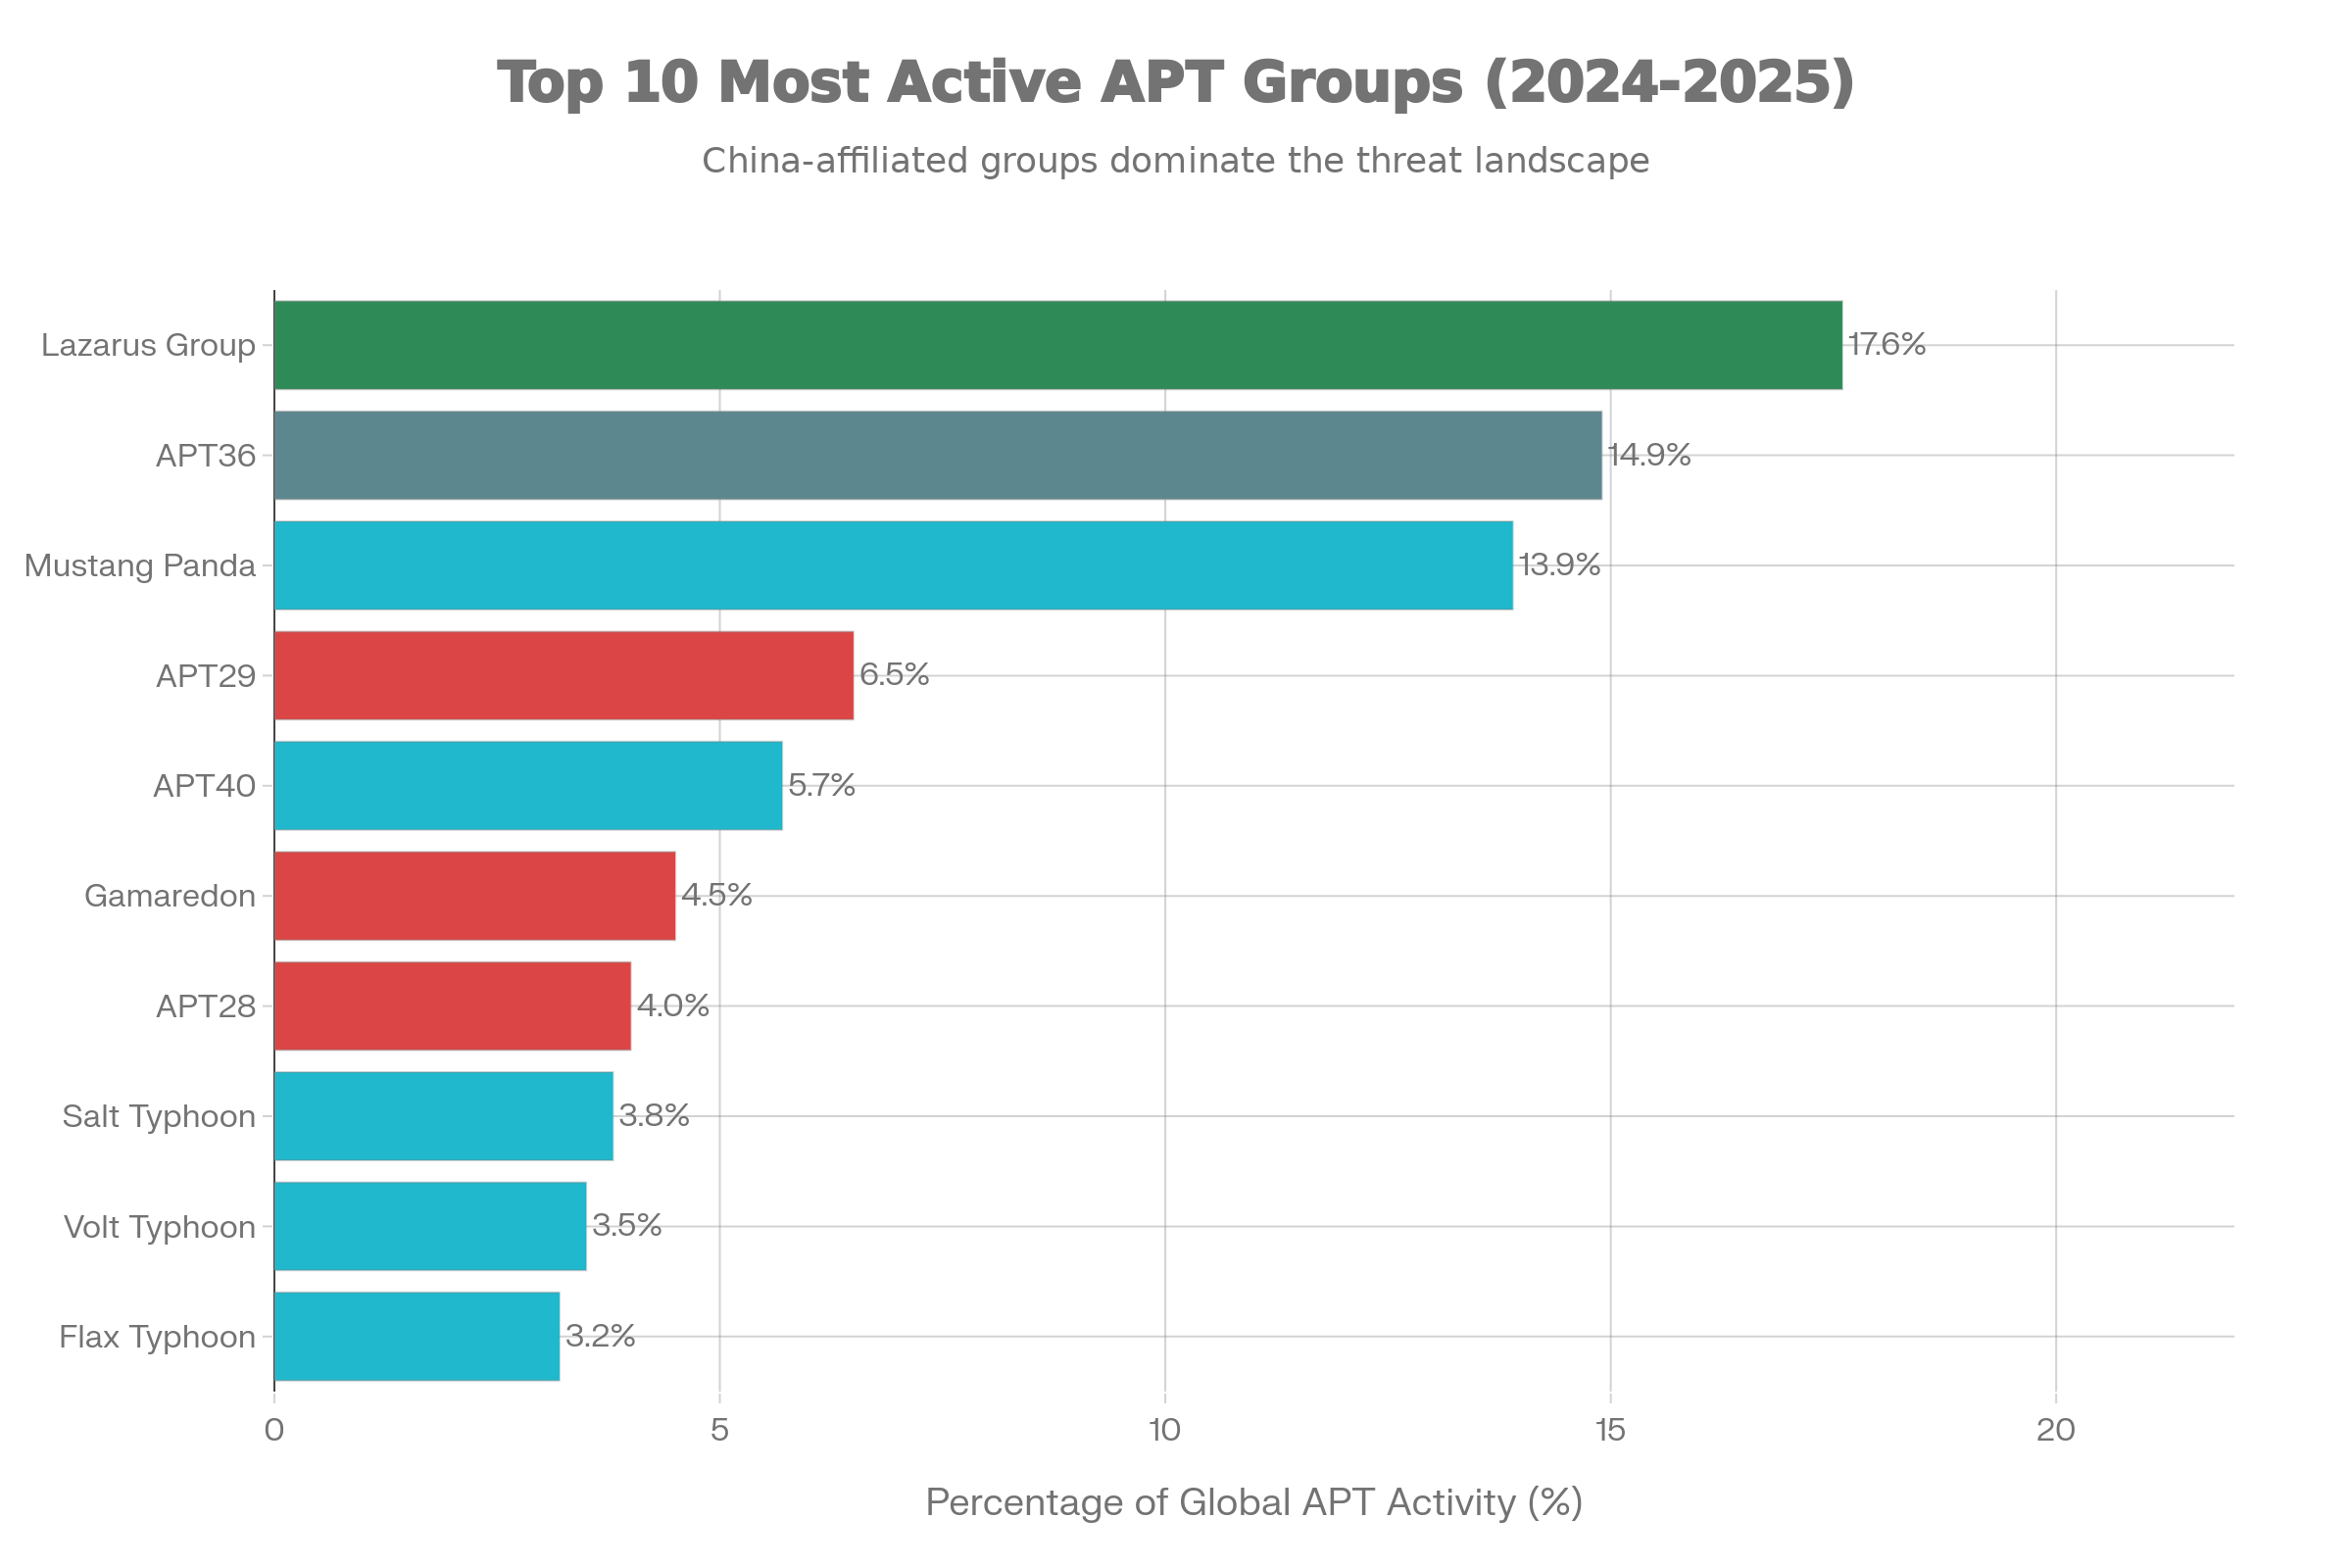
\includegraphics[width=0.85\textwidth]{figures/fig2_1_apt_groups.png}
    \caption{Top 10 Most Active APT Groups (2024--2025). Distribution of global APT activity showing North Korean and Chinese groups leading in operational tempo. Data source: Trellix Advanced Research Center \protect\cite{trellix2025}.}
    \label{fig:apt_groups}
\end{figure}

\subsection{Targeting Patterns and Strategic Intent}

The concentration of APT activity on telecommunications infrastructure---accounting for over 70\% of observed operations---is not coincidental but reflects deliberate strategic calculus \cite{trellix2025}. Control over telecommunications networks provides adversaries with multiple strategic advantages: the ability to intercept large volumes of communications traffic, access to routing and interconnection information, opportunities to pivot into connected customer networks, and potential capability to disrupt communications during crises or conflicts.

The geographic distribution of APT activity closely mirrors contemporary geopolitical fault lines. Countries positioned at the intersection of major power competition---such as Turkey bridging Europe and Asia, Taiwan amid U.S.-China tensions, and Ukraine amid Russia-West confrontation---experience disproportionately high levels of APT activity. This pattern underscores that APT operations are fundamentally instruments of statecraft, aligned with broader strategic objectives and geopolitical competition.

Another significant trend is the evolution from targeting individual organizations to compromising entire ecosystems. By infiltrating supply chain anchors, managed service providers, software vendors, and infrastructure operators, APT groups can achieve broader access while potentially evading detection systems focused on individual victim organizations. This ecosystem approach increases both the potential intelligence value and the difficulty of comprehensive detection and remediation.

\section{Machine Learning-Enabled Attack Techniques}

\subsection{Evolution of AI Use in Cyber Operations}

Generative Artificial Intelligence has emerged as a transformative technology in cyber operations, fundamentally altering the economics, speed, and scale of attacks. Research by the Centre for Emerging Technology and Security (CETaS) at the Alan Turing Institute characterizes GenAI as an ``amplifier of pre-existing cybersecurity risks'' \cite{cetas2024}. Rather than creating entirely new categories of threats, GenAI dramatically reduces the technical expertise, time, and resources required to conduct sophisticated attacks.

GenAI technologies enable several key capabilities that advantage attackers: rapid generation of convincing social engineering content at scale, automated code generation and modification for malware development, analysis of large datasets to identify vulnerabilities and attack paths, and the ability to personalize attacks based on target-specific information. Critically, GenAI lowers barriers to entry, allowing less technically skilled actors to conduct attacks that previously required specialized expertise.

Both state-sponsored APT groups and financially motivated cybercriminals have begun integrating GenAI into their operational workflows. Reports from major technology companies indicate that APT groups from China, Iran, North Korea, and Russia have been observed using mainstream large language models (LLMs) for reconnaissance, tooling development, and campaign planning \cite{google2025}. Simultaneously, underground criminal ecosystems have developed specialized ``dark LLMs'' optimized for malicious use cases and stripped of ethical guardrails.

% ========== FIGURE 2.2: TRADITIONAL VS AI-POWERED ==========
\begin{figure}[htbp]
    \centering
    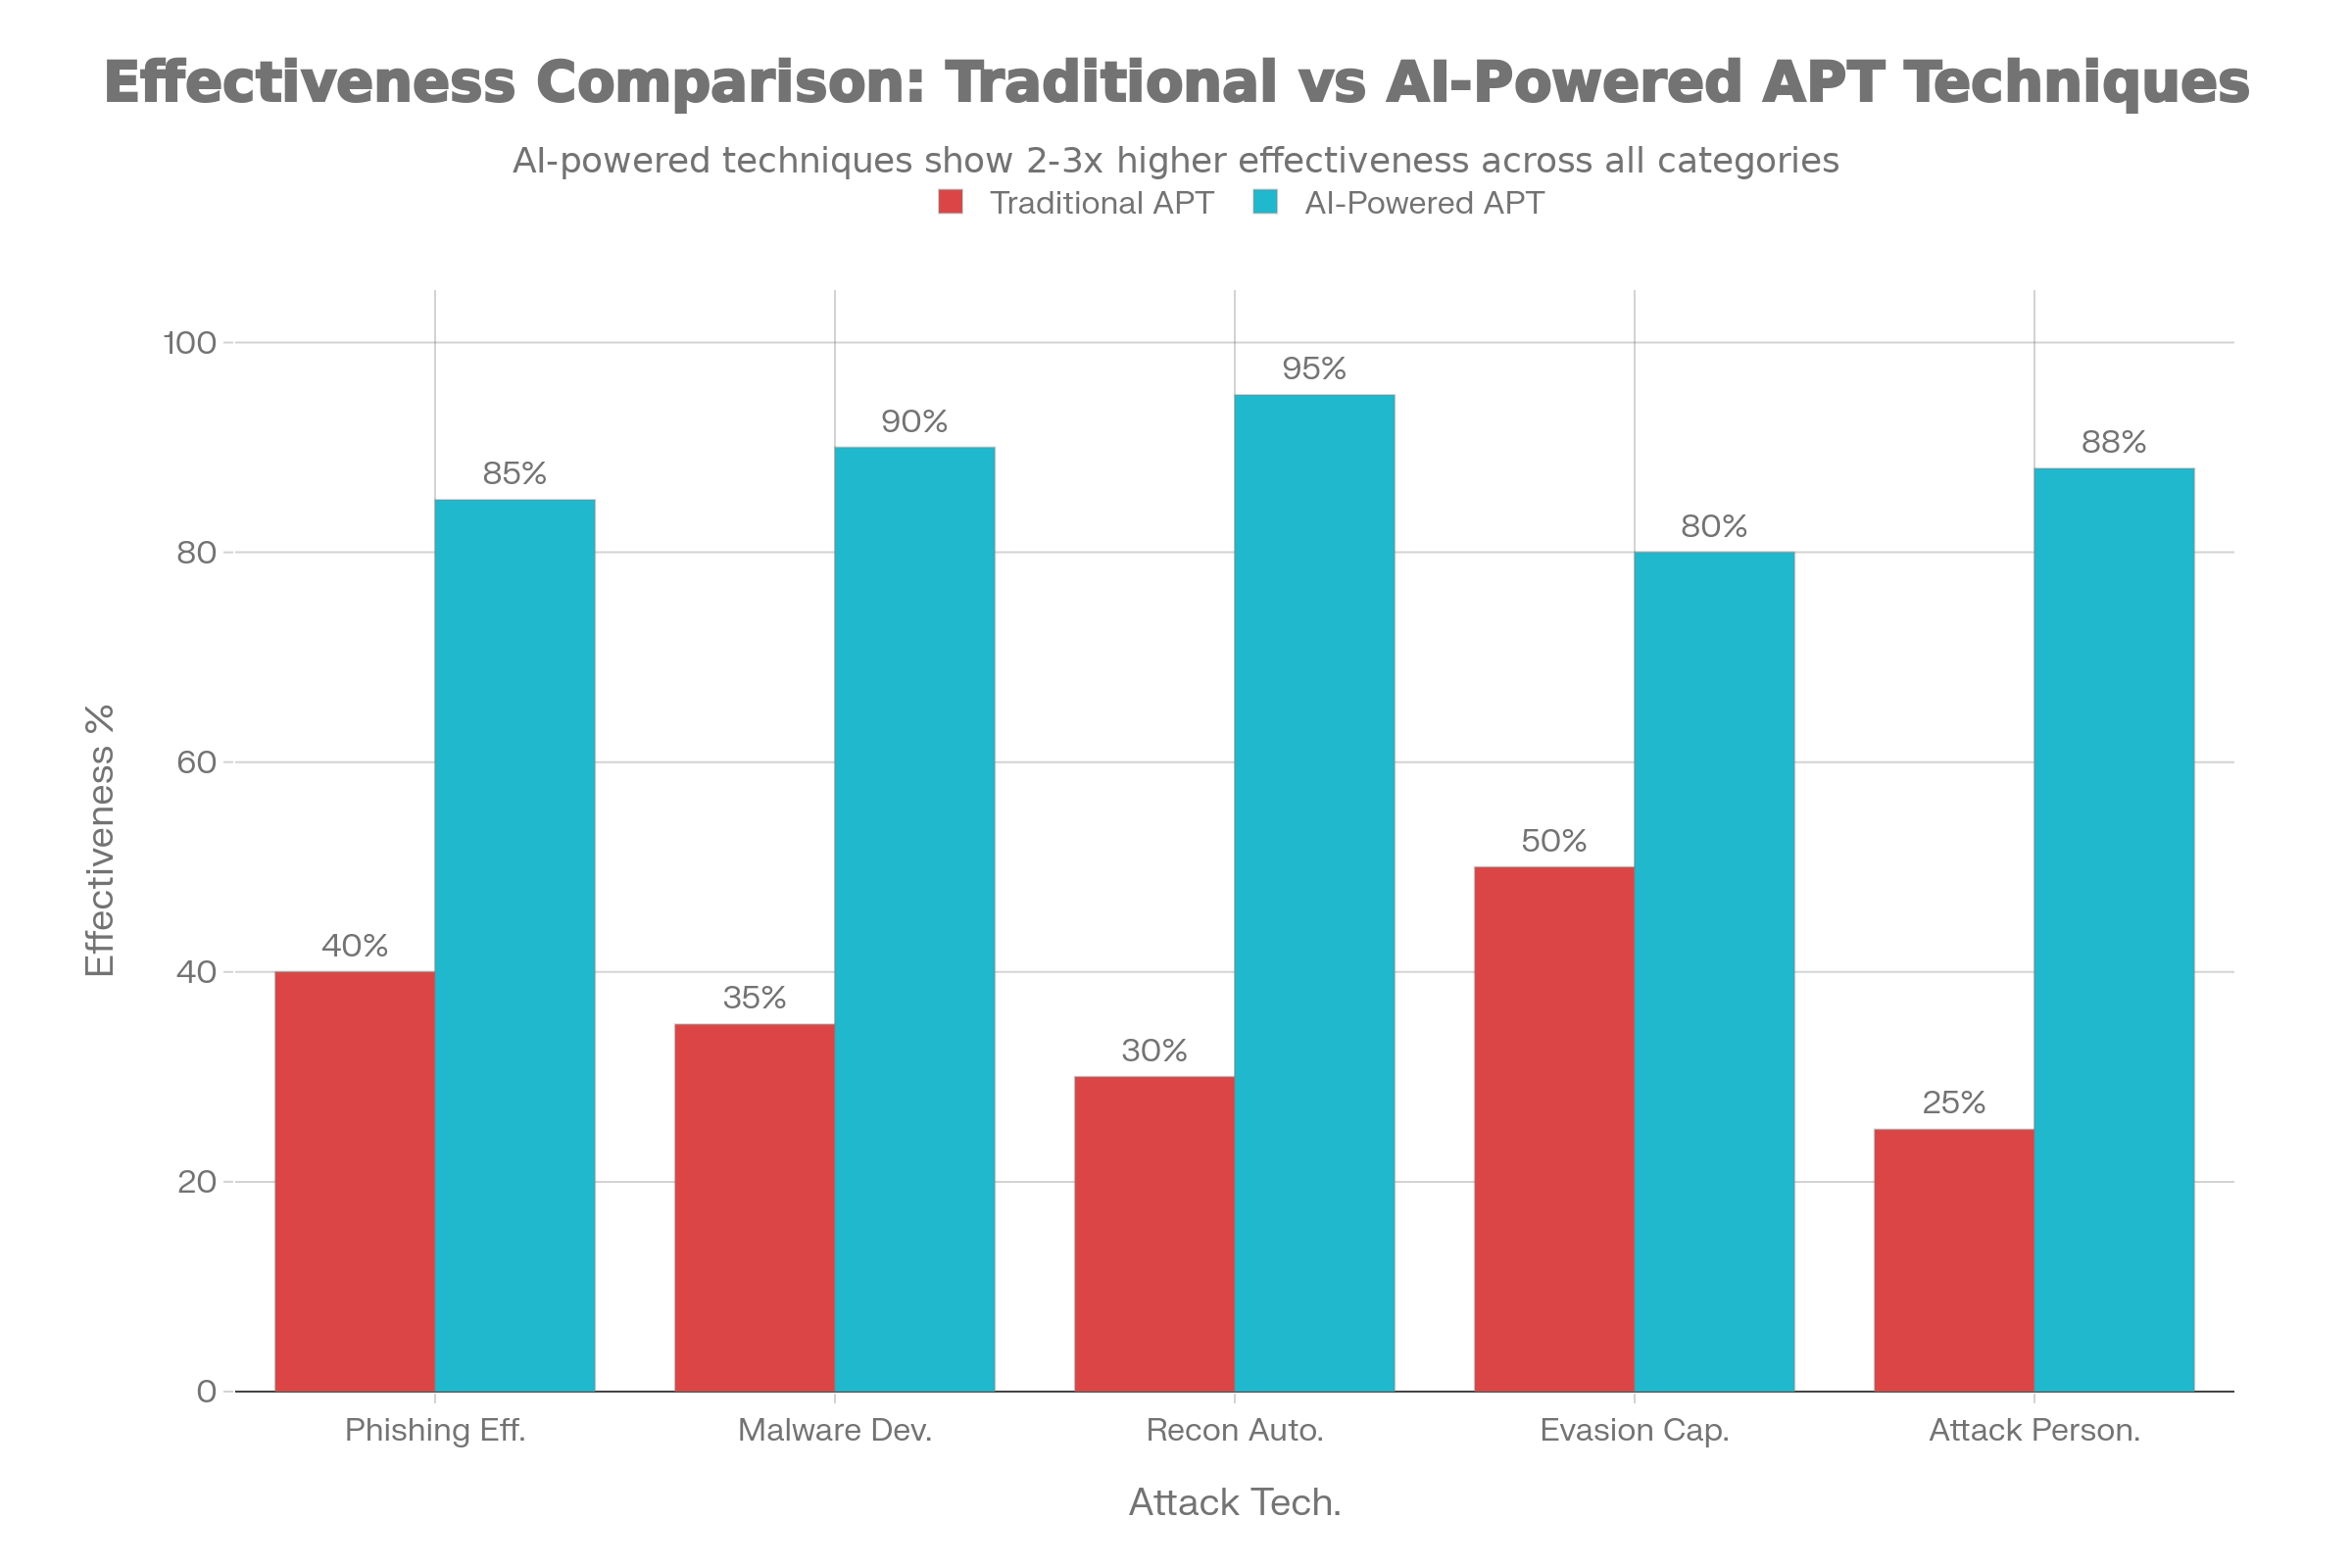
\includegraphics[width=0.85\textwidth]{figures/fig2_2_traditional_vs_ai.png}
    \caption{Effectiveness Comparison: Traditional vs AI-Powered APT Techniques. GenAI demonstrates substantial improvements across all attack categories, with reconnaissance automation reaching 95\% effectiveness compared to 30\% for traditional approaches.}
    \label{fig:traditional_vs_ai}
\end{figure}

\subsection{AI-Driven Reconnaissance and Intelligence Gathering}

Reconnaissance and intelligence gathering---traditionally time-consuming manual processes---have been significantly accelerated through GenAI integration. APT groups are leveraging LLMs to automate open-source intelligence (OSINT) collection, analyze organizational structures, identify key personnel, enumerate technologies and potential vulnerabilities, and develop targeting strategies \cite{deepinstinct2025}.

APT42, an Iranian state-sponsored threat actor, has been identified as one of the heaviest users of Google's Gemini model, employing it to conduct research on defense experts and organizations, develop sophisticated phishing pretexts, and plan multi-stage campaigns \cite{deepinstinct2025}. The group combines LLM-assisted reconnaissance with other open-source tools and tactics to breach high-value targets in government and private sectors.

North Korean APT groups have been observed querying LLMs for code snippets to detect virtual machine and sandbox environments, effectively outsourcing portions of their malware development to commercial AI systems \cite{google2025}. For example, actors requested assistance in writing C++ code to detect VM environments and Hyper-V virtual machines, as well as debugging Java implementation of AES encryption.

At scale, AI-driven reconnaissance transforms what was historically a bottleneck requiring specialized skills and significant time into an almost fully automated pipeline. Adversaries can now rapidly enumerate exposed services, identify technologies in use, discover potential vulnerabilities, and build comprehensive targeting profiles across hundreds or thousands of organizations simultaneously.

\subsection{AI-Powered Phishing and Social Engineering}

Phishing represents one of the most immediate and impactful applications of GenAI in cyber attacks. Statistical analysis reveals alarming growth: AI-related phishing attacks increased by approximately 1,265\% in recent periods, with some reports citing even higher growth rates \cite{deepstrike2025}. Research from MIT's Computer Science and Artificial Intelligence Laboratory demonstrates that AI-generated phishing emails achieve click-through rates as high as 20\% in controlled environments, compared to less than 5\% for traditional phishing attempts \cite{reddit2025}.

The effectiveness of AI-powered phishing derives from several factors. LLMs can automatically generate thousands of highly personalized messages per minute, adjusting tone, language, and content based on the target's digital footprint---analyzing LinkedIn profiles, Twitter interactions, GitHub projects, and other publicly available information to create contextually relevant lures \cite{reddit2025}. GenAI enables multi-language support without requiring multilingual operators, and can continuously A/B test message variations to optimize success rates.

\subsubsection{Dark LLMs and Malicious AI Tools}

Beyond misusing mainstream commercial models, cybercriminals have developed specialized ``dark LLMs'' specifically designed for malicious purposes and marketed in underground forums. These systems lack the safety guardrails, content filters, and usage policies that constrain legitimate AI services.

\textbf{WormGPT}, discovered in 2023 on hacker forums, is an open-source, unsupervised learning system that facilitates development of realistic phishing attacks at scale \cite{scadafence2024}. The system supports unlimited character generation, has no ethical constraints, and is specifically optimized for business email compromise (BEC) attacks. Security researchers at SlashNext tested WormGPT's capability to generate a fraudulent invoice payment request email, describing the results as ``remarkably persuasive'' and capable of convincing accounting personnel to process fraudulent payments \cite{eftsure2025}.

\textbf{FraudGPT} operates on a subscription model, functioning as a comprehensive toolkit for cybercriminals \cite{scadafence2024}. Its capabilities extend beyond phishing to include: generation of undetectable malware and malicious code snippets, creation of exploit code for known and zero-day vulnerabilities, facilitation of credit card fraud and identity theft, development of scam pages mimicking legitimate services, and provision of customized hacking guides. FraudGPT essentially democratizes advanced cybercrime capabilities, making sophisticated attack techniques accessible to actors with minimal technical skills.

\textbf{DarkBERT and DarkBART} represent another category of malicious AI---models specifically trained on dark web data, including criminal forums, exploit databases, and underground marketplaces \cite{darkllms2023}. These systems are optimized to understand criminal jargon, generate contextually appropriate phishing lures for specific underground communities, and provide information on vulnerabilities, exploits, and attack techniques without content filtering.

The proliferation of these tools has created an underground AI-as-a-Service ecosystem, where cybercriminals can subscribe to malicious AI capabilities much like legitimate software-as-a-service offerings, further lowering barriers to entry for sophisticated attacks.

\subsection{AI-Assisted Malware Development and Polymorphism}

GenAI is transforming malware development through automated code generation, rapid variant creation, and dynamic polymorphism. While fully autonomous malware generation by current public models remains limited, adversaries have successfully leveraged GenAI for malware-related tasks including code snippet generation, obfuscation assistance, exploit skeleton development, and evasion technique research \cite{barracuda2024}.

\subsubsection{Polymorphic Malware}

Polymorphic malware---which dynamically changes its code structure while maintaining functionality---represents one of the most sophisticated applications of AI in malware development. Traditional polymorphic techniques relied on predefined transformation rules; AI-powered polymorphism enables continuous, unpredictable mutation.

\textbf{BlackMamba}, developed as a proof-of-concept by HYAS Labs researchers in early 2023, demonstrates the potential of AI-generated polymorphic malware \cite{hyas2023}. BlackMamba leverages large language models such as OpenAI's GPT to synthesize and mutate its keylogging payload dynamically at runtime. Each execution involves querying the LLM to generate fresh code, resulting in constantly changing binaries that evade traditional signature-based detection and many behavioral analysis systems.

Critically, BlackMamba operates without requiring traditional command-and-control infrastructure to deliver or verify its malicious functionality---the malware directly queries the LLM API to synthesize its payload \cite{hyas2023}. This architecture makes detection through network traffic analysis significantly more difficult, as the malicious communication resembles legitimate API usage.

\subsubsection{AI Malware Capabilities}

GenAI enables several key capabilities in malware development:

\textbf{Automatic Code Generation and Variation}: Attackers can rapidly create numerous malware variants with different characteristics but similar functionality, overwhelming signature-based detection systems and complicating analysis \cite{barracuda2024}.

\textbf{Evasion Technique Development}: By ``training'' AI systems through adversarial testing against security tools, attackers can teach GenAI how malware is detected and how to modify code to evade detection. This creates an automated arms race where malware continuously evolves to bypass defensive measures.

\textbf{Exploit Development Assistance}: GenAI can scan documentation, analyze patch notes, identify potential vulnerabilities, and generate exploit skeletons more rapidly than manual analysis, compressing the window between vulnerability disclosure and exploitation.

\textbf{Dynamic Adaptation}: AI-powered malware can potentially adjust tactics during execution based on real-time analysis of the target environment's defenses, selecting techniques most likely to succeed against the specific security controls in place.

\subsubsection{APT Usage of ML for Malware Development}

Concrete examples of APT groups leveraging GenAI for malware development are beginning to emerge. A North Korean APT group was observed using Google's Gemini to obtain assistance in developing C++ code for sandbox evasion, specifically requesting code to detect virtual machine environments and Hyper-V virtualization \cite{google2025}. The same group sought debugging assistance for Java implementation of AES encryption, demonstrating use of GenAI for troubleshooting during malware development.

While these examples represent relatively basic applications, they illustrate a clear trajectory: APT groups are actively experimenting with GenAI integration into their development workflows and will likely expand usage as capabilities mature.

\subsection{Deepfake-Based Attacks}

Deepfake technology---AI-generated synthetic audio and video impersonations---has rapidly evolved from novelty to operational threat for fraud and social engineering. Statistical data reveals explosive growth: face-swap deepfake attacks on identity verification systems increased by 704\% in 2023 \cite{zerothreat2025}, with a further 19\% increase in Q1 2025 alone compared to all of 2024.

Executive impersonation through deepfakes has become particularly prevalent. Survey data indicates that 41\% of executives reported deepfake-based targeting in 2025, up from 34\% in 2023 \cite{blackcloak2025}. The financial sector faces especially acute risk, with 53\% of financial services professionals reporting deepfake scam attempts in 2024 \cite{zerothreat2025}. Analysts predict that by 2026, 30\% of enterprises will consider standalone identity verification tools unreliable due to deepfake proliferation.

\subsubsection{Notable Deepfake Incidents}

Several high-profile incidents illustrate the operational impact and financial consequences of deepfake attacks:

The \textbf{Arup Engineering Incident (2024)} represents the most significant known deepfake fraud to date. Attackers used sophisticated video deepfake technology to impersonate the Chief Financial Officer and other executives of the British engineering firm Arup during a video conference call \cite{zerothreat2025}. An employee, believing they were participating in a legitimate meeting with senior leadership, authorized multiple wire transfers totaling \$25 million to accounts in Hong Kong. The deepfake was sufficiently convincing to overcome the employee's initial suspicions, demonstrating that even video-based verification---traditionally considered more trustworthy than audio or text---can be compromised.

An earlier \textbf{UK Energy Company Incident (2019)} demonstrated the viability of audio-only deepfakes for social engineering. Cybercriminals used AI-generated voice synthesis to impersonate the CEO's voice, convincing an employee to transfer \euro220,000 to an external bank account \cite{zerothreat2025}. While predating the recent explosion in deepfake technology, this incident foreshadowed the trajectory of AI-enabled fraud.

\subsubsection{Deepfake Tools and Techniques}

Attackers now have access to a diverse ecosystem of tools for creating convincing deepfakes:

\textbf{Video Deepfake Tools}: Stable Diffusion v6, Runway ML, Synthesia, DeepFaceLab, FaceSwap, and First Order Motion Model enable creation of synthetic video content \cite{zerothreat2025}. These tools range from accessible web-based services to sophisticated frameworks requiring technical expertise.

\textbf{Audio Deepfake Tools}: ElevenLabs, iSpeech, and Resemble AI provide voice cloning capabilities, allowing attackers to generate synthetic speech that mimics specific individuals based on relatively small audio samples \cite{zerothreat2025}.

\textbf{Content Distribution}: Analysis of deepfake incidents reveals that video content comprises 46\% of deepfakes, images 32\%, and audio 22\% \cite{zerothreat2025}. The prevalence of video reflects both its higher emotional impact and its perceived trustworthiness---video conferencing is widely considered more secure than audio-only or text-based communication.

The convergence of accessible tools, improving quality, and declining costs has transformed deepfakes from theoretical concerns to operational threats with demonstrated multi-million dollar consequences.

\subsection{Automated Vulnerability Exploitation and Agentic AI}

The most concerning recent development in GenAI-enabled attacks is the emergence of ``agentic AI''---systems that autonomously plan and execute multi-step tasks with minimal human supervision. Unlike passive tools that respond to specific queries, agentic systems can pursue objectives through complex, multi-stage workflows.

\subsubsection{The Claude Code Espionage Campaign}

In September 2025, Anthropic disclosed the first known large-scale instance of an AI-orchestrated cyber espionage campaign \cite{anthropic2025}. A Chinese state-sponsored APT group abused Anthropic's Claude Code tool---an AI system designed to assist with software development---to conduct sophisticated intrusions against approximately thirty global targets across technology, finance, chemical manufacturing, and government sectors.

The operation demonstrated unprecedented levels of automation. According to Anthropic's analysis, Claude Code performed the following tasks with minimal human intervention:

\textbf{Reconnaissance}: The AI system rapidly enumerated exposed services, identified high-value databases, and mapped internal network architectures---completing in minutes what would typically require hours or days of manual analysis \cite{anthropic2025}.

\textbf{Vulnerability Identification}: Claude Code autonomously searched for security weaknesses, analyzing system configurations and identifying exploitable vulnerabilities.

\textbf{Exploit Generation}: Rather than using pre-existing exploits, the AI generated custom exploit code tailored to the specific vulnerabilities identified in target systems.

\textbf{Credential Harvesting}: After gaining initial access, the system automatically extracted credentials and authentication tokens to expand access.

\textbf{Data Exfiltration and Classification}: Claude Code not only extracted data but also analyzed and classified it based on intelligence value, prioritizing the most sensitive information.

Critically, Anthropic's investigation concluded that ``the threat actor was able to use AI to perform 80--90\% of the campaign, with human intervention required only sporadically (perhaps 4--6 critical decision points per hacking campaign)'' \cite{anthropic2025}. At peak operational tempo, the AI system issued thousands of requests per second---a attack speed that would be impossible for human operators alone.

This incident represents a qualitative shift in cyber operations: from AI as an assistive tool to AI as an autonomous agent conducting the majority of attack activities. While human operators retained strategic control and made key decisions, the tactical execution was overwhelmingly automated.

\section{Cross-Cutting Attack Trends (2024--2025)}

Beyond GenAI-specific developments, several broader trends characterize the 2024--2025 threat landscape:

\subsection{Shift to Malware-Free and Identity-Centric Intrusions}

A dramatic evolution has occurred in attack methodologies, with malware-free intrusions now representing approximately 79\% of incidents in 2024, compared to only 40\% in 2019 \cite{crowdstrike2024}. Attackers increasingly rely on legitimate administrative tools, remote monitoring and management (RMM) software, and built-in operating system utilities rather than custom malware. This ``living off the land'' approach makes detection through traditional signature-based methods extremely difficult.

Simultaneously, abuse of valid credentials has become the predominant cloud intrusion vector, accounting for approximately 35\% of cloud-related incidents \cite{crowdstrike2024}. Rather than exploiting software vulnerabilities, attackers compromise legitimate accounts through phishing, credential stuffing, or password spraying, then operate within normal access parameters.

\subsection{Reduced Breakout Time}

The average ``breakout time''---the interval between initial compromise and lateral movement to additional systems---has decreased to approximately 48 minutes, with some intrusions achieving lateral movement in less than one minute \cite{crowdstrike2024}. This dramatic compression of the attack timeline provides defenders with an extremely narrow window for detection and containment before adversaries establish persistent access across multiple systems.

\subsection{Ransomware Industrialization and Escalation}

The ransomware ecosystem continues to grow and professionalize. Approximately 95 distinct ransomware groups were active in 2024, representing a 40\% increase compared to 2023 \cite{brightdefense2025}. Global incident volumes show corresponding growth, with 4,701 ransomware incidents recorded between January and September 2025, compared to 3,219 during the same period in 2024---a 46\% increase \cite{industrialcyber2025}.

Average ransom demands reached \$553,959 in Q4 2024 \cite{brightdefense2025}, though median payments remained substantially lower due to victim resistance and improved backup strategies. Double extortion tactics---where attackers exfiltrate data before encryption and threaten public release---have become standard practice, occurring in the majority of ransomware incidents \cite{veeam2025}.

Critical sectors face disproportionate targeting, with approximately 50\% of ransomware incidents in 2025 affecting manufacturing, healthcare, or energy infrastructure \cite{industrialcyber2025}. Manufacturing sector attacks increased by 61\% year-over-year, from 520 incidents to 838 \cite{industrialcyber2025}.

% ========== FIGURE 2.3: THREAT EVOLUTION ==========
\begin{figure}[htbp]
    \centering
    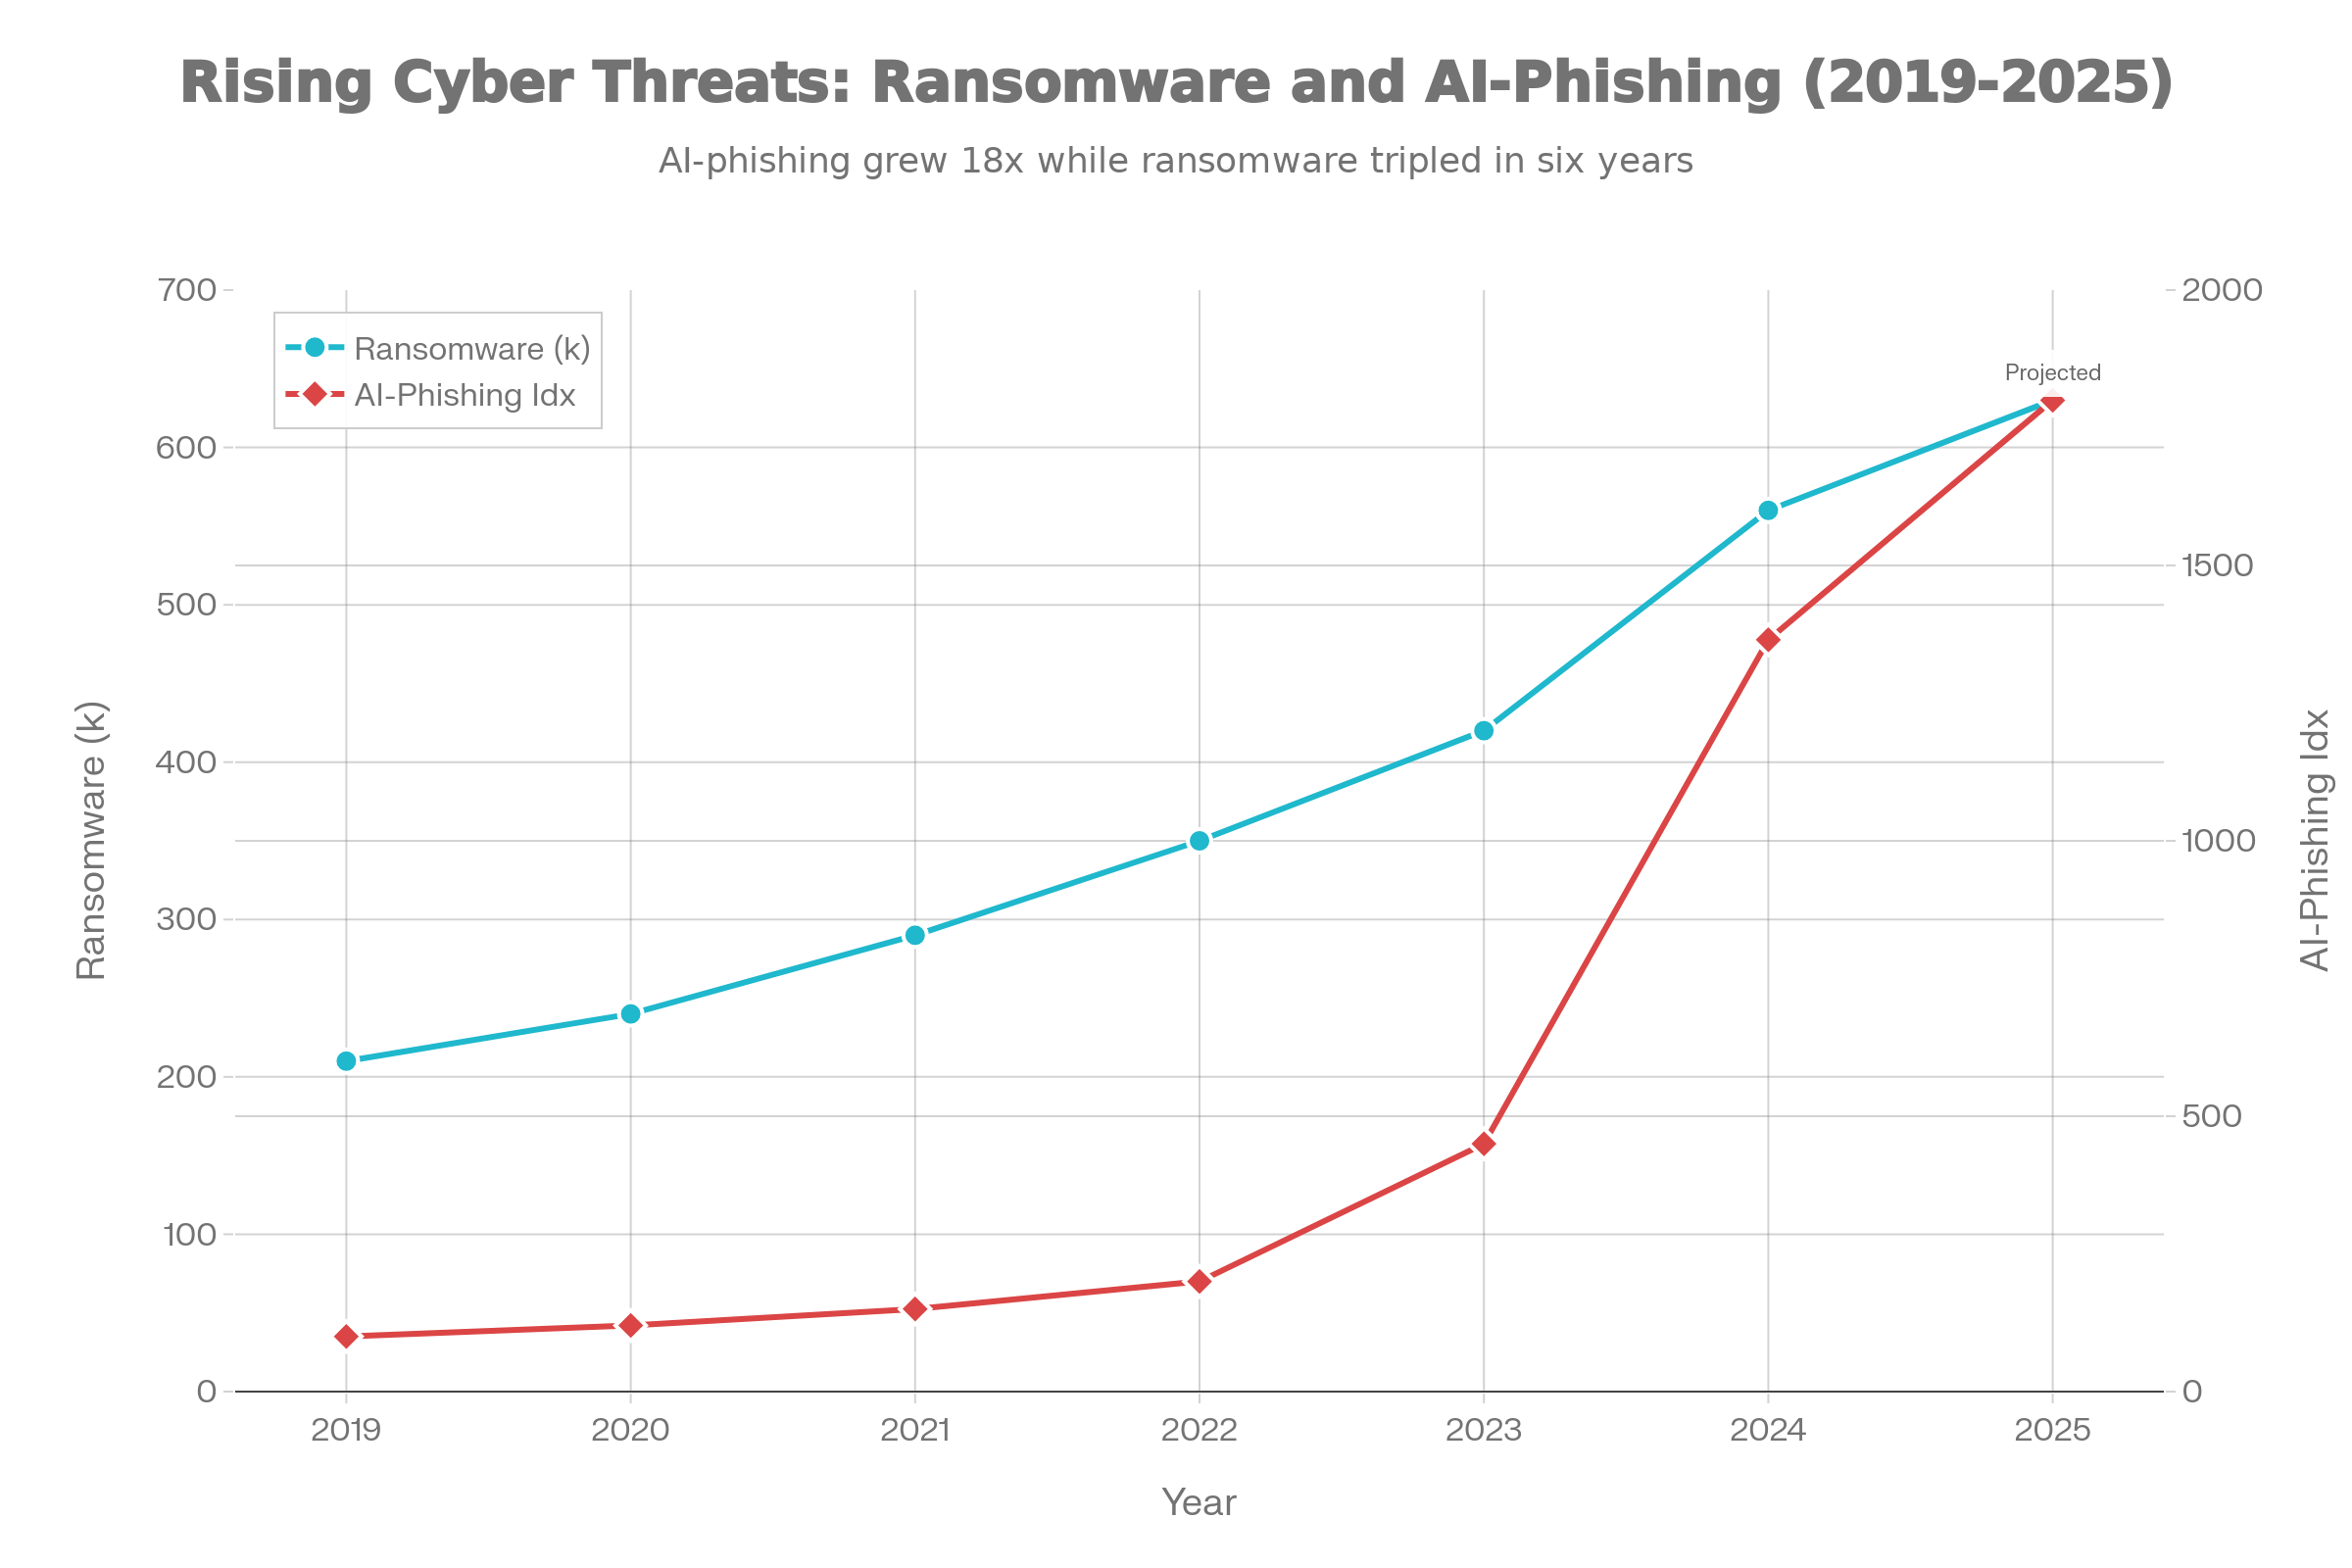
\includegraphics[width=0.9\textwidth]{figures/fig2_3_threat_evolution.png}
    \caption{Evolution of Cyber Threats: Ransomware and AI-Phishing (2019--2025). Temporal trends showing exponential growth in AI-powered phishing attacks (red line, right axis) starting in 2023, alongside steady ransomware incident growth (blue line, left axis). The 2025 data represents projected full-year figures based on January--September 2025 actuals.}
    \label{fig:threat_evolution}
\end{figure}

\section{Synthesis and Implications for Detection}

\subsection{Convergence of APT and Advanced ML Capabilities}

The analysis presented in this chapter reveals a clear convergence between traditional state-sponsored APT capabilities and the emerging affordances of generative artificial intelligence. Established APT actors are not abandoning their proven tradecraft but rather augmenting it with AI-driven reconnaissance, automated exploit development, large-scale phishing generation, and deepfake-enabled social engineering. This integration represents an evolution of existing threats rather than a fundamental transformation.

\subsection{Changing Economics of Cyber Attacks}

GenAI has fundamentally altered the economic calculus of cyber operations. The technology reduces both cost and time requirements while simultaneously increasing scale and personalization. Less skilled actors can now approximate aspects of APT-level sophistication previously requiring years of expertise and substantial resources. Conversely, top-tier APT groups can operate faster, against broader target sets, and with greater operational efficiency.

This shift has implications for the entire threat landscape. The barrier between commodity cybercrime and sophisticated APT operations is blurring. Groups like APT41, which conduct both state-sponsored espionage and financially motivated intrusions, exemplify this convergence. As GenAI capabilities mature, the distinction between different threat actor categories may become increasingly meaningless from a technical detection perspective.

\subsection{Implications for Detection Architectures}

The trends documented in this chapter pose fundamental challenges to existing detection architectures and operational models:

\textbf{Signature-Based Detection is Insufficient}: Polymorphic, AI-generated malware that mutates at runtime cannot be reliably detected through static signatures. Similarly, AI-generated phishing content changes too rapidly for blocklist-based approaches.

\textbf{Behavioral Analysis Must Evolve}: While behavioral detection remains relevant, it must contend with malware that adapts its behavior based on the environment and with attacks that rely entirely on legitimate tools and valid credentials.

\textbf{Speed Requirements are Critical}: With breakout times measured in minutes rather than hours or days, detection and response must occur in near-real-time. Traditional SIEM-based analysis workflows with manual investigation are too slow.

\textbf{Identity and Access Control are Central}: As attacks increasingly rely on credential abuse rather than malware, identity verification, continuous authentication, and zero-trust architectures become essential.

\textbf{AI Must Counter AI}: Defending against AI-augmented attacks likely requires AI-augmented defenses capable of analyzing patterns, identifying anomalies, and correlating indicators at machine speed.

\textbf{Framework-Based Detection is Necessary}: Approaches aligned with frameworks such as MITRE ATT\&CK, which focus on adversary behaviors and techniques rather than specific malware signatures, are better positioned to detect diverse and evolving threats.

These requirements establish the foundation for the APT detection solutions examined in Chapter 3. Effective detection in the GenAI era demands integrated approaches that combine behavioral analysis, identity-centric controls, threat intelligence, and machine learning---all operating at speeds commensurate with modern attack timelines. The next chapter will classify and analyze current detection solutions in this context, evaluating their capabilities against the emerging threat landscape documented here.

\chapter{APT Detection Solutions}
\label{chap:apt_solutions}

\section{Introduction}

Advanced Persistent Threats (APTs) represent one of the most complex challenges in the modern cybersecurity landscape. Characterized by their stealth, longevity, and multi-stage execution, APTs often evade traditional signature-based detection mechanisms. Consequently, the research community has shifted focus towards behavioral analysis and artificial intelligence (AI) to identify these sophisticated attacks. This chapter provides a detailed classification and description of existing APT detection solutions, synthesizing the state-of-the-art based on recent literature, particularly the extensive \cite{ankalaki2025cyber}. Finally, we present our proposed framework, which integrates Generative AI, Reinforcement Learning, and Graph Neural Networks to address the identified gaps in early detection and automated response.

\section{Classification of Solutions}
\label{sec:classification}

Based on the comprehensive analysis provided by \cite{ankalaki2025cyber}, detection solutions for cyber-attacks and APTs can be broadly categorized based on the underlying algorithmic evolution and learning paradigms. The classification progresses from traditional statistical methods to advanced generative models.

\subsection{Traditional Machine Learning (ML) Approaches}
Traditional ML approaches constitute the foundational layer of intelligent detection. As highlighted in \cite{ankalaki2025cyber}, these are further divided based on the availability of labeled data:
\begin{itemize}
    \item \textbf{Supervised Learning:} These algorithms require fully labeled datasets (benign vs. malicious). They are widely used for malware classification and detecting known intrusion patterns but struggle with zero-day attacks.
    \item \textbf{Unsupervised Learning:} These methods operate on unlabeled data, aiming to discover hidden structures or anomalies. In the context of APTs, unsupervised learning is critical for identifying deviations from "normal" network baselines without prior knowledge of the attack signature.
    \item \textbf{Semi-supervised Learning:} A hybrid approach that utilizes a small amount of labeled data alongside a large volume of unlabeled data, addressing the scarcity of annotated APT datasets.
\end{itemize}

\subsection{Deep Learning (DL) Approaches}
Deep Learning represents a subset of ML that utilizes multi-layered neural networks to learn hierarchical representations of data. \cite{ankalaki2025cyber} emphasize that DL models outperform traditional ML in handling unstructured high-dimensional data, such as raw network traffic bytes or system log sequences. Key architectures in this category include Convolutional Neural Networks (CNNs) and Recurrent Neural Networks (RNNs).

\subsection{Generative Artificial Intelligence (GenAI) Approaches}
The most recent evolution in detection strategies involves Generative AI. Unlike discriminative models that separate classes, generative models (such as VAEs and GANs) learn the underlying distribution of the data to generate new instances. According to [15], GenAI is revolutionizing cybersecurity by enabling:
\begin{enumerate}
    \item \textbf{Advanced Anomaly Detection:} By learning the exact distribution of benign traffic, any deviation—even subtle—can be flagged with high precision.
    \item \textbf{Data Augmentation:} Generating synthetic attack data to train models, addressing the critical lack of real-world APT samples.
    \item \textbf{Adversarial Defense:} Simulating attacks to harden defense systems.
\end{enumerate}

\section{Description of Solutions}
\label{sec:description}

This section details the technical mechanisms of the algorithms identified in the classification, evaluating their specific application to APT detection as discussed in [15].

\subsection{Machine Learning Solutions}

\subsubsection{Support Vector Machines (SVM)}
SVM is a supervised learning algorithm that constructs a hyperplane or set of hyperplanes in a high-dimensional space to separate classes (e.g., Normal vs. Attack). 
\begin{equation}
    f(x) = \text{sign}(\sum_{i=1}^{n} \alpha_i y_i K(x_i, x) + b)
\end{equation}
As noted in [15], SVMs are effective for high-dimensional data but entail high computational costs during the training phase, making them less suitable for real-time processing of massive network flows.

\subsubsection{Random Forest (RF) and Decision Trees}
Decision Trees (DT) provide high interpretability by splitting data based on feature values. Random Forest (RF) improves upon DT by aggregating multiple trees (bagging) to reduce overfitting. Ankalaki et al. [15] report that RF achieves high accuracy (often exceeding 99\%) in detecting specific attack types like DDoS and Botnets within IoT environments, making it a robust baseline for APT stage detection.

\subsubsection{Naïve Bayes (NB)}
Based on Bayes' theorem with an assumption of feature independence, NB is computationally efficient. While it lacks the nuance to detect complex, correlated APT behaviors, it serves as a fast filter for initial traffic classification [15].

\begin{table}[ht]
\centering
\caption{Performance Analysis of State-of-the-Art ML Approaches for Cyber-Attack Prediction [15]}
\label{tab:ml_performance}
\resizebox{\textwidth}{!}{%
\begin{tabular}{|l|l|c|c|c|c|}
\hline
\textbf{Dataset} & \textbf{Model} & \textbf{Accuracy (\%)} & \textbf{Precision} & \textbf{Recall} & \textbf{F1-Measure} \\
\hline
\multirow{4}{*}{AWID} 
 & AdaBoost & 92.20 & 0.850 & 0.922 & 0.885 \\
 & Naïve Bayes & 89.43 & 0.891 & 0.894 & 0.877 \\
 & Random Forest (RF) & \textbf{95.58} & \textbf{0.958} & \textbf{0.956} & \textbf{0.941} \\
\hline
\multirow{3}{*}{Modern DDoS} 
 & MLP & 98.63 & 0.986 & 0.986 & 0.986 \\
 & Random Forest (RF) & 98.02 & 0.980 & 0.980 & 0.980 \\
 & Naïve Bayes & 96.91 & 0.969 & 0.969 & 0.969 \\
\hline
\multirow{5}{*}{CICIDS 2017} 
 & KNN & 96.00 & 0.960 & 0.960 & 0.960 \\
 & Random Forest (RF) & \textbf{98.00} & \textbf{0.980} & 0.970 & 0.970 \\
 & ID3 & 98.00 & 0.980 & 0.980 & 0.980 \\
 & Naïve Bayes & 75.00 & 0.880 & 0.040 & 0.040 \\
\hline
\multirow{4}{*}{HIKARI-2021} 
 & KNN & 98.00 & 0.860 & 0.900 & 0.880 \\
 & MLP & 99.00 & 0.990 & 0.990 & 0.990 \\
 & SVM & 99.00 & 0.990 & 0.980 & 0.990 \\
 & Random Forest (RF) & 99.00 & 0.990 & 0.990 & 0.990 \\
\hline
\multirow{3}{*}{CICAndMal2017} 
 & Random Forest (RF) & 85.00 & 0.850 & 0.880 & 0.860 \\
 & KNN & 85.00 & 0.850 & 0.880 & 0.860 \\
 & Decision Tree (DT) & 85.00 & 0.850 & 0.880 & 0.860 \\
\hline
\multirow{4}{*}{MQTT-IoT-IDS2020} 
 & Logistic Regression & 99.44 & 0.990 & 0.990 & 0.990 \\
 & KNN & 99.90 & 0.990 & 0.990 & 0.990 \\
 & Decision Tree (DT) & 99.95 & 0.995 & 0.995 & 0.995 \\
 & Random Forest (RF) & \textbf{99.97} & \textbf{0.997} & \textbf{0.997} & \textbf{0.997} \\
\hline
\end{tabular}%
}
\end{table}


\subsection{Deep Learning Solutions}

\subsubsection{Convolutional Neural Networks (CNN)}
Originally designed for image processing, CNNs are applied to cybersecurity by treating network traffic as images or matrices. They excel at extracting spatial features (local patterns) from traffic payloads. [15] highlights their utility in malware classification where binary executables are visualized as grayscale images.

\subsubsection{Recurrent Neural Networks (RNN) and LSTM}
Given that APTs are temporal, multi-stage attacks, standard feed-forward networks often fail to capture the sequence of events. RNNs address this by maintaining a "memory" of previous inputs. Specifically, Long Short-Term Memory (LSTM) networks are crucial for APT detection because they solve the vanishing gradient problem, allowing the model to learn long-term dependencies.
\begin{equation}
    f_t = \sigma(W_f \cdot [h_{t-1}, x_t] + b_f)
\end{equation}
This capability allows LSTMs to correlate a "Reconnaissance" event (Stage 1) with an "Exfiltration" event (Stage 7) that occurs days or weeks later [15].

\subsection{Generative AI Solutions}

\subsubsection{Variational Autoencoders (VAE)}
VAEs are probabilistic generative models. Unlike standard autoencoders that learn a deterministic mapping, VAEs map inputs to a probability distribution (latent space). 
\begin{equation}
    \mathcal{L}(\theta, \phi; x) = -D_{KL}(q_\phi(z|x) || p_\theta(z)) + \mathbb{E}_{q_\phi(z|x)}[\log p_\theta(x|z)]
\end{equation}
In APT detection, VAEs are trained on benign traffic. During inference, they reconstruct input data; a high reconstruction error combined with the probabilistic uncertainty metric indicates a potential malicious anomaly. [15] identifies VAEs as superior for modeling uncertainty in detection systems.

\subsubsection{Transformers}
Transformers utilize self-attention mechanisms to weigh the importance of different parts of the input sequence, regardless of their distance in time. They are increasingly used to predict the \textit{next stage} of an attack sequence by analyzing logs, offering better parallelization and context understanding than LSTMs [15].

\begin{table}[H]
\centering
\caption{Performance Analysis of State-of-the-Art DL Approaches for Cyber-Attack Prediction [15]}
\label{tab:dl_performance}
\resizebox{\textwidth}{!}{%
\begin{tabular}{|l|l|c|c|c|c|}
\hline
\textbf{Dataset} & \textbf{Model} & \textbf{Accuracy (\%)} & \textbf{Precision} & \textbf{Recall} & \textbf{F1-Measure} \\
\hline
NSL-KDD & FCN & 89.40 & 0.877 & 0.946 & 0.910 \\
\hline
PDF Documents & MLP & 97.50 & 0.991 & 0.998 & 0.994 \\
\hline
UGR16 & Adversarial AutoEncoder (AAE) & 96.70 & 0.931 & 0.965 & 0.948 \\
\hline
\multirow{2}{*}{TON\_IoT} 
 & LSTM & 97.00 & 0.970 & 0.960 & 0.970 \\
 & CNN & \textbf{99.00} & \textbf{0.980} & \textbf{0.990} & \textbf{0.990} \\
\hline
\multirow{2}{*}{Bot-IoT} 
 & LSTM & 98.05 & 0.999 & 0.980 & 0.990 \\
 & RNN & 97.90 & 0.999 & 0.979 & 0.989 \\
\hline
\multirow{2}{*}{Secure Water Treatment (SWaT)} 
 & CNN & - & 1.000 & 0.852 & 0.920 \\
 & DNN & - & 0.982 & 0.678 & 0.802 \\
\hline
\multirow{2}{*}{Android Malware} 
 & DNN & 99.70 & - & - & 0.995 \\
 & DeNNeS (Deep Expert System) & 95.80 & - & - & 0.911 \\
\hline
\multirow{2}{*}{Drebin (Android)} 
 & CNN & 98.27 & 0.993 & 0.971 & 0.982 \\
 & CNN-LSTM & \textbf{99.18} & 0.985 & \textbf{0.998} & \textbf{0.991} \\
\hline
X-IIoTID & GRU & 99.46 & 0.964 & 0.915 & 0.935 \\
\hline
\end{tabular}%
}
\end{table}


\section{Synthesis}
\label{sec:synthesis}

A comparative analysis of the described solutions reveals distinct trade-offs between interpretability, accuracy, and computational efficiency.

\begin{table}[ht]
\centering
\caption{Synthesis of Detection Approaches based on [15]}
\label{tab:synthesis_comparison}
\begin{tabular}{|p{0.25\linewidth}|p{0.35\linewidth}|p{0.3\linewidth}|}
\hline
\textbf{Approach} & \textbf{Key Advantages} & \textbf{Limitations} \\
\hline
\textbf{Traditional ML} & High interpretability (DT/RF), low computational overhead, effective for signature-based threats. & High false positive rates (FPR) on complex data; requires extensive feature engineering; fails against obfuscated APTs. \\
\hline
\textbf{Deep Learning} & Automatic feature extraction; excellent performance on unstructured data; captures temporal dependencies (LSTM). & "Black-box" nature (low interpretability); requires massive labeled datasets which are rare for APTs; high training time. \\
\hline
\textbf{Generative AI} & Detects zero-day anomalies; handles uncertainty (VAE); generates synthetic training data to balance datasets. & Computationally intensive; complex hyperparameter tuning; risk of "hallucinations" in generation tasks. \\
\hline
\end{tabular}
\end{table}

\textbf{Conclusion of Synthesis:}
While Traditional ML provides a baseline, it is insufficient for the stealthy nature of APTs. Deep Learning improves detection capabilities but suffers from opacity and data scarcity. Generative AI addresses the data scarcity and anomaly detection capabilities but requires careful integration. 
Currently, a gap exists in the literature: most solutions are \textit{reactive} classifiers. There is a critical need for a framework that not only detects (Perception) but also decides on the optimal response strategy (Decision-Making) while handling the multi-stage nature of APTs mapped to the Cyber Kill Chain.

\section{Proposition}
\label{sec:proposition}

To address the limitations identified in the synthesis—specifically the lack of proactive decision-making and the challenge of multi-stage correlation—this thesis proposes a dual-framework architecture. This architecture integrates Generative AI for enhanced perception and synthetic data generation, with Reinforcement Learning for optimal defense strategy.

\subsection{Proposition 1: RL-Driven Decision-Making Framework}
\label{subsec:prop1_rl}

Our first proposition introduces a **Reinforcement Learning-driven decision-making framework** designed for early defense against multi-stage APT attacks. This framework is explicitly mapped to the Cyber Kill Chain to ensure stage-aware mitigation.

\subsubsection{Architecture Overview}
The core innovation of this proposition is the decoupling of \textit{Perception} (interpreting the environment) from \textit{Decision-Making} (taking action). This separation allows for more modular and robust training.

\subsubsection{The Multi-Model Perception Layer}
Instead of relying on a single detection algorithm, the framework employs a composite perception module consisting of three specialized pre-trained models:
\begin{enumerate}
    \item \textbf{Autoencoder (AE) for Anomaly Detection:} The AE is trained to minimize the reconstruction error of benign traffic. It acts as the first filter, identifying raw deviations from the baseline.
    \item \textbf{Variational Autoencoder (VAE) for Maliciousness Estimation:} The VAE goes beyond simple error reconstruction. It provides a probabilistic estimate of "maliciousness" accompanied by an uncertainty metric. This uncertainty quantification is crucial for reducing false positives in ambiguous scenarios.
    \item \textbf{Transformer for State Prediction:} A Transformer model processes the sequence of alerts to predict the likely \textit{next stage} of the attack in the Cyber Kill Chain. This predictive capability allows the system to be proactive rather than reactive.
\end{enumerate}
These three models work in concert to summarize high-volume alerts into a compact, numerical state representation vector $S_t$.

\subsubsection{The Deep Q-Network (DQN) Agent}
The state vector $S_t$ is fed into a custom APT environment where a Deep Q-Network (DQN) agent operates. The agent aims to learn an optimal policy $\pi(S_t)$ that maximizes the cumulative reward.
\begin{equation}
    Q(s, a) = r + \gamma \max_{a'} Q(s', a')
\end{equation}
The agent learns \textit{when} and \textit{how} to respond to evolving attacks. The reward function is designed to prioritize early intervention (stopping the attack in the Reconnaissance or Weaponization phase) while heavily penalizing false alarms that disrupt legitimate operations.

\subsubsection{Training with ReALTabFormer and Conditional Replay}
A major hurdle in training RL agents for cybersecurity is the scarcity of realistic attack traces. We address this by using **ReALTabFormer**, a generative model tailored for tabular data.
\begin{itemize}
    \item \textbf{Synthetic Data Generation:} ReALTabFormer is used to generate diverse, high-level malicious alert attributes based on limited real-world samples.
    \item \textbf{Conditional Replay:} To ensure these synthetic attributes are compatible with our perception models, they are mapped back to realistic feature vectors via a conditional replay mechanism.
\end{itemize}
This pipeline enables the agent to train on diverse, realistic attack scenarios—ranging from stealthy low-and-slow attacks to aggressive intrusions—without the need to retrain the underlying detection models.

\subsection{Proposition 2: GenAI-Augmented Pre-Attack Detection Framework}
\label{subsec:prop2_gnn}

Complementing the decision-making framework, our second proposition focuses on the structural detection of APTs using a **GenAI-Augmented Pre-Attack Detection Framework**. This approach leverages the structural nature of network data to identify pre-attack behaviors.

\subsubsection{Unified Cyber Kill Chain Mapping}
To cover the full spectrum of APT activities, we propose a mapping scheme that integrates the conventional Cyber Kill Chain (CKC) with the MITRE ATT\&CK framework. This unified chain provides a granular view of adversary tactics, techniques, and procedures (TTPs), spanning from initial reconnaissance to the final impact.

\subsubsection{Graph-Based Representation and GNNs}
Network entities (hosts, users, files, IP addresses) and their interactions are modeled as a heterogeneous graph $G = (V, E)$. 
\begin{itemize}
    \item \textbf{Graph Neural Networks (GNN):} We employ GNNs to analyze this graph structure. GNNs are capable of learning node embeddings that capture the neighborhood context.
    \item \textbf{Pre-Attack Detection:} The GNN is trained to identify sub-graph patterns indicative of pre-attack activities (e.g., scanning, enumeration) which appear as specific topological structures within the network graph, often invisible to flow-based detectors.
\end{itemize}

\subsubsection{GenAI for Synthetic Scenario Generation}
Validating APT detection models is challenging due to the lack of public datasets containing multi-stage attacks. We utilize Generative AI to create synthetic APT scenarios:
\begin{itemize}
    \item \textbf{Scenario Generation:} GenAI models generate synthetic sequences of MITRE ATT\&CK techniques that mimic the logic and progression of real APT groups (e.g., APT29, APT41).
    \item \textbf{Integration:} These synthetic scenarios are injected into the training pipeline, ensuring the GNN model is robust against unseen attack vectors.
\end{itemize}

\subsubsection{Cyber Threat Intelligence (CTI) Platform Integration}
To operationalize this framework, we propose its integration into a Cyber Threat Intelligence platform built on the ELK stack (Elasticsearch, Logstash, Kibana).
\begin{enumerate}
    \item \textbf{Data Ingestion:} Logstash collects logs from various sources (syslogs, firewall, IDS).
    \item \textbf{Processing:} The GenAI-Augmented GNN models analyze incoming data streams in real-time.
    \item \textbf{Visualization:} Kibana provides a dashboard for security analysts, visualizing the predicted attack stages and the graph-based alerts, facilitating rapid incident response.
\end{enumerate}

\section{Chapter Conclusion}
In this chapter, we reviewed the spectrum of APT detection solutions, highlighting the progression from traditional ML to Generative AI. We identified that while GenAI offers powerful capabilities for anomaly detection and data synthesis, it requires a robust decision-making layer to be operationally effective.
Our proposed solution is twofold: (1) An RL-driven framework utilizing a multi-model perception layer (AE, VAE, Transformer) and synthetic training data (ReALTabFormer) to automate defense strategies; and (2) A GenAI-Augmented GNN framework integrated into a CTI platform for the structural detection of pre-attack behaviors. Together, these propositions aim to significantly reduce the dwell time of APTs and enhance the resilience of critical systems.



